%Typeset using XeLaTeX

\documentclass[10pt,a4paper]{book}
\usepackage{mathtools,amssymb,amsthm}
%\usepackage{phonetic}
\usepackage{fancyhdr}
\usepackage[pass]{geometry}
\usepackage{fontspec}
%\usepackage{xunicode}
%\usepackage{xltxtra}
%\usepackage{xgreek}
\setmainfont[Mapping=TeX-text]{Times New Roman}
\usepackage{hyperref}
%\usepackage{color}
\usepackage[Glenn]{fncychap}
\ChNameVar{\bfseries\Large}
%\usepackage{tabularx}
%\usepackage[normalem]{ulem}

\usepackage{enumerate}
\usepackage{tikz}
\usepackage{multicol}
\usepackage{natbib}
\usepackage{algorithm}
\usepackage{algpseudocode}

\renewcommand{\maketitle}{
	\begin{titlepage}
		\newgeometry{left=4cm, top=2.3cm, bottom=2.3cm}
		\hbox{\mbox{\hspace{-1.3cm}}
			\vrule depth 0.98\textheight
			\mbox{\hspace{1cm}}
			\vtop{
				\vspace{2cm}
				\begin{flushleft}
					\huge{\bf Pricing Games in Heterogeneous Parallel Networks\\}
					\vskip3cm
					\Large  Thomas Pappas\\
					AL1.18.0011\\
					\vskip3cm
					\begin{minipage}{7.5cm}
						\begin{flushleft}
							\normalsize {\it {\bf Examination committee:}\\
								Dimitris Fotakis, School of Electrical and Computer Engineering, National Technical University of Athens.\\
								Professor's name, Department or School, Institution.\\
								Professor's name, Department or School, Institution.}
						\end{flushleft}
					\end{minipage}
					\hskip0.5cm
					\begin{minipage}{6cm}
						\begin{flushleft}
							\normalsize {\it {\bf Supervisor:}\\
								Dimitris Fotakis, Professor, \\ School of Electrical and Computer Engineering,\\
								National Technical University of Athens.\\
							}
						\end{flushleft}
					\end{minipage}
				\end{flushleft}
				\vskip6cm
				\hskip4.5cm
				\begin{minipage}{5cm}
					\begin{center}
						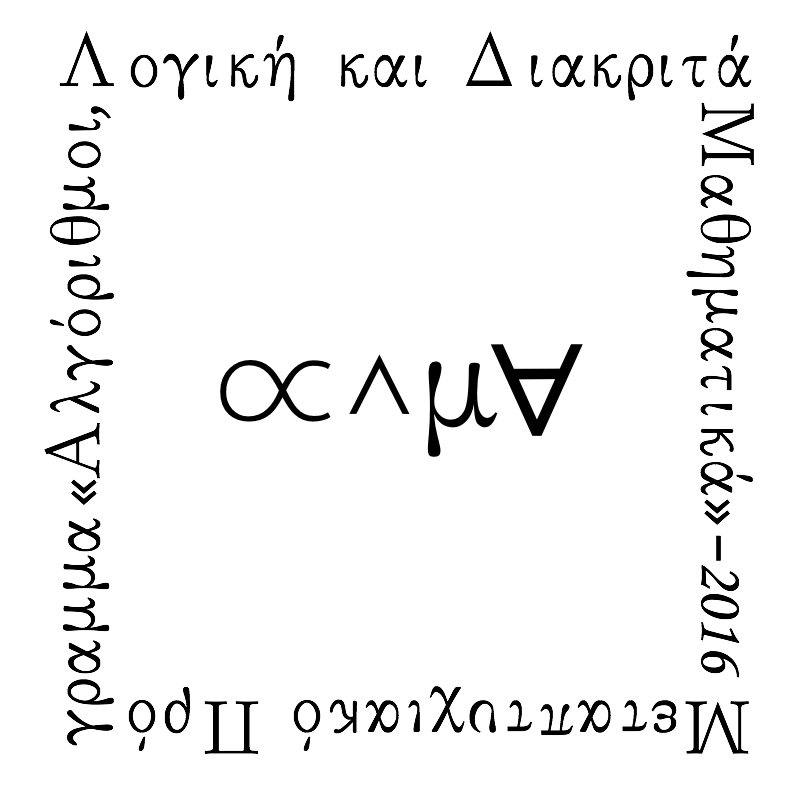
\includegraphics[width=0.8\textwidth]{alma.png}
					\end{center}
		\end{minipage}}}
	\end{titlepage}
}

% Commands for wrapping properly common expressions.
\newcommand{\indeq}[1]{\stackrel{\text{#1}}{=}}
\newcommand{\RightarrowArg}[1]{\stackrel{#1}{\Rightarrow}}
\newcommand{\LeftrightarrowArg}[1]{\stackrel{#1}{\Leftrightarrow}}
\newcommand{\NE}{\mathrm{N.E.}}
\newcommand{\as}{\mathrm{\alpha_s}}
\newcommand{\R}{\mathbb{R}}
\newcommand{\N}{\mathbb{N}}
\newcommand{\Gm}{\mathcal{G}}
\DeclareMathOperator*{\argmax}{arg\,max}
% \newcommand{\Exp}{\mathrm{Exp}}
% \newcommand{\Expect}{{\rm I\kern-.3em E}}

% Theorem structures.
\theoremstyle{definition}
\newtheorem{ex}{}[section]
\newtheorem{definition}{Definition}[chapter]
\newtheorem{theorem}[definition]{Theorem}
\newtheorem{lemma}[definition]{Lemma}
\newtheorem{corollary}[definition]{Corollary}
\theoremstyle{comment}
\newtheorem{example}[definition]{Example}
\newtheorem{claim}[definition]{Claim}

\fancyhead[LO]{\slshape \leftmark}
\fancyhead[RE]{\slshape \rightmark}
\fancyhead[LE]{}
\fancyhead[RO]{}
\fancyfoot[LO,RE]{\tiny{\it}}

% Main document
\begin{document}

\maketitle
\clearpage


\thispagestyle{empty}
\null
\clearpage

\restoregeometry

\thispagestyle{empty}
\pagenumbering{gobble}
\chapter*{Abstract}
In this masters thesis we study a $2$-level game where, on an $n$-link network from a source $s$ to a target $t$, a unit of flow wants to move from $s$ to $t$ using the link with the lowest cost, while the link operators compete for profit by assigning tolls to links and thus creating a toll congestion game.
We examine only affine latencies for the links.
In addition, each flow user responds to tolls in a heterogeneous way, i.e. each player $p$ in the flow has a different time-money sensitivity value, which is described by a distribution function $\alpha(p)$.
We first present some definitions and properties of pricing homogeneous games, heavily based on previous work, and using them as base, we extend them to describe pricing games with heterogeneous users.
We introduce a new term, the sensitivity split function $\as(t)$, defined for any $2$ links of the network as the time-money sensitivity value for which, given a set of tolls $t$, the link costs are equal.
With the help of $\as$ we describe some properties around the selfish behaviour of heterogeneous users for different tolls, as well as prove the existence of bounds for the sensitivity values that are relevant to the game.
Then, arriving at the main body of this study, we investigate the existence of a Nash Equilibrium in the profit game between the link operators for different cases of heterogeneous users.
We show there is no Nash Equilibrium when there are many users with $0$ sensitivity, i.e. players not affected by tolls, so we further assume $\alpha(p) > 0$.
We then investigate cases of fixed distribution functions, which, even though create homogeneous behaviour for the users (making them pseudo-heterogeneous games), help us describe how flow, tolls and equilibria behave as that fixed value changes.
Using all the above, we study step distribution functions, where by limiting our scope to $2$ links, we present strict conditions necessary for the existence or not of a Nash Equilibrium in the profit game between the link operators.
We present and analyse an algorithm to calculate that equilibrium, if it exists, and finish with some discussion about potential future work.
\clearpage

\thispagestyle{empty}
\null
\clearpage

\thispagestyle{empty}
\pagenumbering{gobble}

\chapter*{Συνοψη}
Σε αυτή τη διπλωματική μεταπτυχιακού μελετάμε ένα παίγνιο $2$ επιπέδων όπου, σε ένα δίκτυο με $n$ ακμές από μια πηγή $s$ σε ένα στόχο $t$, μια μονάδα ροής θέλει να μετακινηθεί από το $s$ στο $t$ χρησιμοποιώντας την ακμή με το χαμηλότερο κόστος, ενώ οι διαχειριστές των ακμών ανταγωνίζονται για κέρδος βάζοντας δίοδια στις ακμές και δημιουργώντας έτσι ένα παίγνιο συμφόρησης με διόδια.
Εξετάζουμε μόνο αφινικές καθυστερήσεις για τις ακμές.
Επιπλέον, ο κάθε χρήστης δικτύου αντιδρά στα διόδια με ετερογενή τρόπο, δηλ. ο κάθε παίκτης $p$ στη ροή του δικτύου έχει διαφορετική τιμή ευαισθησίας χρόνου-χρήματος, η οποία περιγράφεται από μια συνάρτηση κατανομής $\alpha(p)$.
Πρώτα παρουσιάζουμε κάποιους βασικούς ορισμούς και ιδιότητες των ομογενών παιγνίων κέρδους, κυρίως βασισμένα σε προηγούμενες δουλειές, και με αυτά ως βάση, τα επεκτείνουμε για να περιγράψουμε παίγνια κέρδους με ετερογενείς χρήστες.
Εισαγάγουμε έναν νέο όρο, τη συνάρτηση διαχωρισμού ευαισθησίας $\as(t)$, ορισμένη για οποιεσδήποτε $2$ ακμές του δικτύου ως η τιμή ευαισθησίας χρόνου-χρήματος για την οποία, δωσμένων σετ διοδίων $t$, τα κόστη των $2$ ακμών είναι ίσα.
Με τη βοήθεια της $\as$ θα περιγράψουμε μερικές ιδιότητες γύρω από την εγωιστική συμπεριφορά των ετερογενών χρηστών για διαφορετικά διόδια, καθώς και θα αποδείξουμε την ύπαρξη άνω φράγματος για τις τιμές ευαισθησίας που αφορούν το παίγνιο.
Στη συνέχεια, φτάνοντας στο κύριο σώμα αυτής της έρευνας, εξετάζουμε την ύπαρξη ισορροπίας Nash στο παίγνιο κέρδους μεταξύ των διαχειριστών των ακμών για διαφορετικές περιπτώσεις ετερογενών χρηστών.
Δείχνουμε ότι δεν υπάρχει ισορροπία Nash όταν υπάρχουν πολλοί χρήστες με $0$ ευαισθησία, δηλ. παίκτες που δεν επηρρεάζονται από τα διόδια, οπότε στο εξής υποθέτουμε ότι $\alpha(p) > 0$.
Κατόπιν εξετάζουμε περιπτώσεις όπου η συνάρτηση κατανομής είναι σταθερή, η οποίες, αν και δημιουργούν ομογενή συμπεριφορά στους χρήστες (κάνοντάς τα ψευδο-ετερογενή παίγνια), μας βοηθάνε να περιγράψουμε πώς συμπεριφέρονται η ροή, τα διόδια και τα σημεία ισορροπίας όταν αυτή η σταθερή τιμή μεταβάλλεται.
Χρησιμοποιώντας όλα τα παραπάνω, μελετάμε βηματικές συναρτήσεις κατανομής, όπου περιορίζοντας το μοντέλο μας σε στιγμιότυπα $2$ ακμών, παρουσιάζουμε αυστηρές συνθήκες αναγκαίες για την ύπαρξη ή μη σημείου ισορροπίας Nash στο παίγνιο κέρδους μεταξύ των διαχειριστών των ακμών.
Παρουσιάζουμε και αναλύουμε έναν αλγόριθμο για τον υπολογισμό του σημείου ισορροπίας, αν υπάρχει, και κλείνουμε με μια συζήτηση για πιθανή μελοντική δουλειά.

\clearpage

\thispagestyle{empty}
\null
\clearpage

\pagestyle{fancy}

\pagenumbering{roman}
\tableofcontents
\clearpage

\thispagestyle{empty}
\null
\clearpage

\pagenumbering{arabic}


\chapter{Introduction}
\label{chapter:intro}

In this thesis we study a two level game.
On the basis there is a network with 2 nodes $(s, t)$ and $n$ links, each link directed from $s$ to $t$ and weighted by a non-decreasing latency function that defines how the traffic increases as more players flow into that link.
On the lower level, a flow $[0, 1]$ wants to move from $s$ to $t$ using one of the $n$ links and experience minimum latency (traffic).
On the upper level, each link is managed by a different operator who can assign a toll to their link and gain profit proportional to that toll and the flow that ends up using the link.
The tolls impose an additional cost to the flow players, affecting the lower level game, and the link operators compete with each other to maximise their profit.
In our case we will additionally assume that the flow users behave in a heterogeneous way when it comes to tolls, meaning that each player has a different time-money trade-off and thus see the link costs differently.

The structure of this thesis is as such.
We finish this chapter by briefly presenting previous work in this field, all while examining some of the different models and properties that have been researched in the literature so far.
This will also serve as a bridge to Chapter \ref{chapter:preliminaries} were we will set our basis for the rest of the study.
This includes formal definitions of the models and properties we introduced from previous work, as well as some additional -but still basic- properties of the models, with heavy focus on the user's time-money trade-off, captured by a money sensitivity distribution function $\alpha$.

Entering the main body of our work, in Chapter \ref{chapter:split} we introduce a new term regarding any two links of the network, called \textit{money sensitivity split}, which captures the notion of a (potentially non-existent) player whose money sensitivity makes them view the two links as equal.
We will then analyse that notion and provide properties and bounds for its values.
Finally, in the chapter's main result, we prove a general property of heterogeneous network games as, due to the previously found bounds, there might be a portion of users whose sensitivity value can be arbitrarily large without affecting the game.

Having arrived at our main results in this work, in Chapter \ref{chapter:pricing_equilibria} we investigate the pricing competition game between the link operators of a network with heterogeneous users.
We begin by examining a class of games where the distribution function is fixed across all users, which, as we'll formally describe, makes the game \textit{pseudo-heterogeneous}.
Particular interest in the above class is the relation between games with identical setup but with different fixed distribution functions.
We describe and prove some properties for them, and using those we then tackle step distribution functions (where the user sensitivity can take values out of a finite set).
At this point we restrict our model to instances with $2$ links, and provide strict restrictions for equilibrium existence for the pricing competition game.

We conclude this thesis with a short discussion around the main outtakes of this study, while also presenting potential directions for future work.


\section{Related Work}
\label{section:related_work}

Selfish routing is the study of trafficked networks where selfish users seek to optimise their own traffic cost.
The main interest is on instances where all users are content with the traffic they experience and no one wishes to change their strategy, a notion known as a Nash Equilibrium, or equivalently from the work of Wardrop \cite{wardrop_theoretical_1952}, a Wardrop Equilibrium.
Models from this field have been proven extremely useful in solving a variety of real-world problems in economics \cite{pigou1920economics}, transportation \cite{beckmann1956studies}, \cite{wardrop_theoretical_1952} and more, resulting in a vast history in the literature (see \cite{roughgarden2002sr} and \cite{roughgarden2005slpoa} for more references).
It has been well-established, at least as early as 1920 from the work of Pigou \cite{pigou1920economics}, that selfish behavior in congested networks can create (arbitrary) inefficiencies with regard to the total latency experienced by all users.
A long-standing practice to solve these inefficiencies has been to regulate the network by adding tolls to the links, thus altering the cost of the link usage.
A classical result on this is the use of marginal tolls (Beckman et al. \cite{beckmann1956studies}), where each link user is charged a toll corresponding to their externality, i.e. the added congestion effect caused by their participation in the network.
This technique can eradicate the inefficiencies and create optimal flow in the network, however it assumes a strong homogeneity among the users.
Marginal cost pricing has been investigated in networks with heterogeneous users (e.g. Dafermos \cite{dafermos1973toll}), with the resulting payment required by users on same links being different, an unwanted and non-practical approach, which also requires knowledge of the users' sensitivity beforehand.

Congestion games were formally introduced by Rosenthal \cite{Rosenthal1973ACO} who also proved that in those games a pure Nash Equilibrium always exists.
Later, Monterer-Shapely \cite{MONDERER1996124} defined the class of potential games (games where the incentive for all players to change their strategy can be expressed with a global function) and proved that congestion games are equivalent to exact potential games (potential games where a change in strategy from any player alter the potential function the exact way it alters the player's cost).
%One of the major contributions in this field has been the introduction of the Wardrop equilibrium \cite{wardrop_theoretical_1952}, a notion of Nash equilibrium for potential games, where the Wardrop principles provide a framework to describe and analyse those equilibria.
Milchtaich \cite{MILCHTAICH1996111} then investigated different pay-off functions for congestion games, where he showed that even though some best-reply strategies may end up in a cyclic path, there is always a path that leads to Nash equilibrium with pure strategies.

Given the above, with the existence of a Nash equilibrium always existing, later research focused on investigating the quality of an equilibrium by using the notion of \textit{Price of Anarchy}, introduced by Koutsoupias-Papadimitriou \cite{KOUTSOUPIAS200965}.
The Price of Anarchy describes the ratio between a Nash Equilibrium and the most cost-efficient solution, therefore lower values denote a qualitative equilibrium while a lower value denotes a bad one.
Finally, in terms of complexity, Fabrikant et al. \cite{10.1145/1007352.1007445} have shown that calculating a pure Nash Equilibrium for congestion games is PLS-complete in the general case.

Regarding the model properties, there is a multitude of variations in the classical selfish routing model.
Beginning with the network topology, one can distinguish between parallel networks (our case) or series-parallel ones.
In addition the flow traversing through the network can either be atomic (finite number of players, each contributing to congestion equally or weighted) or non-atomic (infinite number of players, each contributing to congestion by an non-influencing infinitesimal amount).
Also the model might admit elastic demand (e.g. \cite{10.1287/moor.1060.0231}, \cite{Hearn1998}), a property where users have a bound on the cost they're willing to pay, making a player potentially not participate in the flow if all link costs are above that bound.

Most work considers homogeneous network users.
Heterogeneity has been studied by Schmeilder \cite{1973JSP.....7..295S} while Milchtaich \cite[Prop $3.3$]{doi:10.1287/moor.25.3.349.12220} has contributed through with work on the more general crowding games, a class of games where the cost assigned to each player is affected only by the number of players selecting the same action (or strategy).
Large crowding games are basically less restrictive $n$-link parallel congestion games.
Also, Cole et al. \cite{10.1145/780542.780618} in their work showed that even general heterogeneous networks can be priced so that an optimal routing emerges while computing those efficient tolls can be done in polynomial time for convex latency functions and distribution functions with only finitely many values.
The latter paper has been one of the main pillars of this thesis.

Discussing more the algorithmic aspect of toll computation, there has been significant research in finding optimal tolls for homogeneous network users.
Marginal cost prices can be computed using convex programming \cite{beckmann1956studies}, while the transportation community has made significant progress in optimising efficient computation and characterisating minimum-latency tolls (\cite{10.1007/978-3-642-59179-2_4}, \cite{Hearn1998}, \cite{Hearn2002}).

Acemoglu and Ozdaglar were the first to introduce pricing competition between link operators to the above model \cite{10.1287/moor.1060.0231}.
They showed that increasing the competition among operators from a monopoly to an oligopoly may reduce the efficiency of the network, achieving tight bounds on the Price of Anarchy.
In a follow-up work \cite{10.1109/JSAC.2007.070812}, they generalised the above by assuming more general topologies where links can also be linked serially (serial-parallel networks).
Correa et al. \cite{correa2018pricing} showed pricing games may not exist, may not be unique and can be arbitrarily inefficient, but regulating the network with toll caps can solve all three issues.
Harkes et al. \cite{Harks_2019} then showed that the same is true for uniform toll caps, which is stronger in practice as toll discrimination is often not allowed.
The latter two papers have also been main pillars of the current work.


\cleardoublepage


\chapter{Preliminaries}
\label{chapter:preliminaries}

In this section we will describe the model utilised throughout this thesis.
If we attempted to call that model by including all of its properties, the result would be a Heterogeneous Non-atomic $n$-link Parallel Network Toll Congestion Pricing Game, so while we will describe each of those properties, we will eventually focus on heterogeneity and the pricing competition, thus calling it a Heterogeneous Pricing Game.

\section*{Non-atomic Parallel Network Games}

We consider a directed graph $G = (\{s, t\}, N)$ where $N = \{1,\dots, n\}$ is a set of parallel links from a source node $s$ to a target node $t$.
For the non-atomic case, there is one unit of traffic that wishes to travel from $s$ to $t$, described as the unit interval $[0, 1]$ endowed with Lebesque measure $\lambda$.
Each point $p \in [0, 1]$ will be called a \textit{player} and will be considered to be non-cooperative and contribute to the traffic by an infinitesimal amount.
As such the decisions of individual players have no effect on the game and it becomes natural to only consider non-zero measure collection of players.

A \textit{flow} is a Lebesque measurable function $f: [0, 1] \rightarrow N$ that describes which link is selected by each player.
It is more intuitive, however, to consider the resulting flow on each link (\textit{flow on paths}), i.e. $x_i = \lambda(\{p \in [0, 1]: f(p) = i\})$.
Hence we get flow as a (stochastic) vector $x = (x_i)_{i \in N}$ where $x_i$ is the total flow on link $i$ with $x_i \geq 0$ and $\sum_{i \in N}x_i = 1$.
The flow then creates congestion on the links, each described by a non-decreasing latency function $(\ell_i)_{i \in N}$ which we assume to be affine.
We denote by $\mathcal{L}_d$ the class of polynomial latency functions with nonnegative coefficients and degree at most $d$, and as such $\mathcal{L}_1$ becomes the class of non-decreasing latency functions.
Finally, the network can also be extended by allowing a set of tolls $t = (t_i)_{i \in N}$ to be assigned to each link, which in turn adds to the effective cost of a player using them.
At this point we should also mention that we will freely use, when needed, the standard game-theoretical notation of $t_{-i} = t \setminus \{t_i\}$.

The above set-up creates a Non-atomic Parallel Network Game with tolls where each player will select the link that minimises their \textit{individual} traffic latency.
We consider two cases where players either react to tolls in a \textit{homogeneous} or a \textit{heterogeneous} manner.

\subsection*{Homogeneous players}

In the homogeneous case all players have an equal reaction to tolls, and therefore the effective cost of a player using link $i$ becomes $\ell_i(x_i) + t_i$.
For a given set of tolls $t$, a flow $x$ is a \textit{Wardrop equilibrium for $t$} if $\forall i, j \in N$ with $x_i > 0$ it holds that
\begin{equation*}
	\ell_i(x_i) + t_i \leq \ell_j(x_j) + t_j
\end{equation*}
In that case, all links with $x_i > 0$ have equal effective costs, i.e. there exists some $K > 0$ such that for all those links $i$ it holds that $\ell_i(x_1) + t_i = K$.
From a well-known result from Beckman et al. \cite{beckmann1956studies} and Dafermos and Sparrow \cite{1363388843888284416}, such and an equilibrium for $t$ exists, is unique with regard to costs and can be described by the following inequality.
\begin{lemma}
	\label{lemma:wardrop_equilibrium}
	A flow $x$ is a Wardrop equilibrium for $t$ if and only if for all feasible flows $x^\prime$,
	\[\sum_{i \in N} (\ell_i(x_i) + t_i) \cdot (x_i - x_i^\prime) \leq 0\]
\end{lemma}

The notion of uniqueness under costs is important in order to acknowledge that a given flow on paths can be achieved by many player-link assignments, since the users can be put arbitrarily on the links, as long as each link is receiving the same total traffic.

We can therefore denote by $x(t)$ the flow occurring on that unique up to costs equilibrium for a given set of toll $t$.
If $t = 0^N$ then the equilibrium is called the \textit{Wardrop equilibrium}.
It's also worth noting that looking at Lemma \ref{lemma:wardrop_equilibrium}, we can see that what actually matters, with regard to the flow, is the relative difference among the tolls, and not their actual values.
To demonstrate this, if we consider an arbitrary $c \in \R_+$ and tolls $t^\prime = t + c$ then for the same flow $x$ and any other flow $x^\prime$ the sum becomes
\begin{flalign*}
	\sum_{i \in N} (\ell_i(x_i) + t_i + c) (x_i - x_i^\prime) &= \sum_{i \in N} (\ell_i(x_i) + t_i) (x_i - x_i^\prime) + c \left(\sum_{i \in N} x_i - \sum_{i \in N} x_i^\prime\right) \\
	&= \sum_{i \in N} (\ell_i(x_i) + t_i) (x_i - x_i^\prime) \leq 0
\end{flalign*}
which makes $x$ the Wardrop equilibrium for $t^\prime$ as well.
The last equality holds because $x_i, x_i^\prime$ are flows of the network and therefore $\sum_{i \in N} x_i = \sum_{i \in N} x_i^\prime = 1$.
Also, this reasoning is still valid for $c < 0$ as long as $t_i + c \ge 0$ for all $i \in N$, or in other words, as long as $c \ge -\min_{i \in N}{t_i}$.

With this observation we can see that the case of $t = 0^N$ is equivalent to any toll instance such that $t_1 = t_2 = \dots = t_n$.
We will therefore simplify our notation and write $t = 0$ when talking about the game without tolls, though we will in fact mean the entire class $\{t = (c)_{i \in N}, c \in \R_+\}$.

Finally for affine latencies we can calculate $x(t)$ by following the same reasoning as \cite[Prop $3.1$]{Harks_2019}.
For $\ell_i(x_i) = a_i x_i + b_i$ with $a_i > 0, b_i \geq 0$ and $t \in \R_+^{|N|}$, define $N(t) = \{i \in N | x_i(t) > 0\}$.
Since $x(t)$ is an equilibrium for $t$ then for all $i \in N(t)$ we get $\ell_i(x_i) + t_i = K$ for some common effective cost $K$.
By also using the fact that $\sum_{j \in N(t)} x_i = 1$ we solve the equations with regard to $K$ and eventually get for all $i \in N(t)$
\begin{equation}
	\label{eq:homogeneous_x_i}
	x_i(t) = \frac{1 + \sum_{j \in N(t)}\frac{b_j + t_j - b_i - t_i}{a_j}}{\sum_{j \in N(t)}\frac{a_i}{a_j}}
\end{equation}

\subsection*{Heterogeneous players}

In the heterogeneous case, each player $p$ reacts differently to tolls, presumably due to different time-money trade-off values.
We describe this by adding a money sensitivity weight $\alpha(p)$ on the toll costs experienced by a player, making them see the cost of a link with flow $x_i$ and toll $t_i$ as $c_i(p) = \ell_i(x_i) + \alpha(p) \cdot t_i$.
For a flow $x$ and tolls $t$, each player considers their costs experienced across all links and then selects to use the one (or one of potentially many) with the lowest cost. 
By also assuming that the players are sorted by money sensitivity, we can describe their heterogeneity by defining a non-decreasing function $\alpha: [0, 1] \rightarrow [0, +\infty]$.
We call $\alpha$ a \textit{distribution function}.
Even though the definition does allow functions that are not upper bounded with $\alpha(1) = +\infty$, we will always assume that $\alpha$ is finite on $[0, 1)$.
%Finally, we will assume that $\alpha(0) > 0$, since, as we'll see in more detail in Lemma \ref{lemma:a_0_0}, allowing many players close to $0$ breaks the pricing game.

We can therefore define an instance of a Heterogeneous Pricing Game as the tuple $(N, \ell, \alpha)$, with $N = \{1, 2, \dots, n\}$ the links of the network, $\ell = (\ell_i)_{i \in N}$ the affine latency functions for each link and $\alpha$ the non-decreasing distribution function.
With all the above we can again define a Nash equilibrium for the game if $\forall i \in N$ and $\forall p \in [0, 1]$ it holds that
\[c_{f(p)}(p) \leq c_i(p)\]
Existence of an equilibrium is guaranteed by the more general results of Schmeidler \cite[Thm 2]{1973JSP.....7..295S}, while uniqueness with regard to costs is covered by Milchtaich \cite[Prop 3.3]{doi:10.1287/moor.25.3.349.12220} (see Related Work \ref{section:related_work}); for a more detailed coverage of those look at the definitions and propositions of Cole et al. \cite[\S2]{10.1145/780542.780618}.
We can therefore also extend the definition of $x(t)$, being the Nash Equilibrium for $t$, similarly as in the homogeneous case.

We will now prove a general property of parallel networks which captures the relationship between latencies and tolls.
It is trivial for homogeneous games that higher tolls create lower latencies on their respective links, but for the heterogeneous case it is not straightforward so we'll prove it.

\begin{lemma}
	\label{lemma:latencies_tolls}
	Let $(N, \ell, \alpha)$ a Heterogeneous Parallel Game with tolls $t$ and flow $x(t)$ the Nash equilibrium for $t$.
	It holds for all $i, j \in N$ with $x_i(t), x_j(t) > 0$ that
	\begin{enumerate}[(i)]
		\item $\ell_i(x_i(t)) < \ell_j(x_j(t))$ iff $t_i > t_j$
		\item $\ell_i(x_i(t)) = \ell_j(x_j(t))$ iff $t_i = t_j$
		\item $\ell_i(x_i(t)) > \ell_j(x_j(t))$ iff $t_i < t_j$
	\end{enumerate}
\end{lemma}

\begin{proof}
	We will prove $(i)$ and the rest follow similarly.
	For the left-to-right direction we assume that $\ell_i(x_i(t)) < \ell_j(x_j(t))$.
	If we also assume that $t_i \le t_j$, then for all players $p$ we get $\ell_i(x_i(t)) + \alpha(p) \cdot t_i < \ell_j(x_j(t)) + \alpha(p) \cdot t_j \Rightarrow c_i(p) < c_j(p)$.
	Since $x_j(t) > 0$ there exist players $p_j$ on link $j$ for which $c_{f(p_j)}(p_j) = c_j(p_j) > c_i(p_j)$, which is a contradiction since $x(t)$ is a Nash equilibrium.
	The opposite direction is also proved similarly.
\end{proof}

This property shows us that for a given $t \in \R_+^{|N|}$, if we order the links according to decreasing toll values, then the same link order will have latencies ordered in increasing values (and vice-versa).
It is then easy to show that the players using each such link are also ordered with regard to their $\alpha$ values in increasing order.
Therefore a given set of tolls can define an ordering of links where $t_1 \ge t_2 \ge \dots \ge t_n$ and $\ell_1(x_1(t)) \le \ell_2(x_2(t)) \le \dots \le \ell_n(x_n(t))$, while if we were to pick player representatives from each link with positive flow $p_1, p_2, \dots, p_k$, we also get $\alpha(p_1) \le \alpha(p_2) \le \dots \le \alpha(p_k)$.
Note that the ordering is unique only when the inequalities are strict, as had we had $t_i = t_j$ for any $i, j \in N$ then $i$ and $j$ can be ordered arbitrarily.
If $t = 0$ then all links can be ordered arbitrarily, which is why when comparing $t$ with $0$ we will assume the ordering is the same for simplicity.
We continue with the following lemma which describes a property for the last link in such an ordering.

\begin{lemma}
	\label{lemma:xn_xn0_lower_bound}
	Let $(N, \ell, \alpha)$ a heterogeneous parallel game.
	For tolls $t \in \R_+^{|N|}$ consider the links in decreasing toll ordering.
	It holds that $x_n(t) \ge x_n(0)$.
\end{lemma}

\begin{proof}
	Consider $t^\prime = t - t_n$.
	From assumption we have $t_n = \min_{i \in N} t_i$, which makes $t^\prime \in \R_+^{|N|}$ with $t_n^\prime = 0$.
	Since the flow equilibrium $x(t)$ is dependent only on the toll differences, we get $x(t) = x(t^\prime)$.
	Also, by now comparing $t^\prime$ with $t = 0$, no additional tolls have been added to link $n$, making $x_n(t^\prime) \ge x_n(0)$.
	The proposition follows naturally from the previous two statements.
\end{proof}

Finally we need to discuss about toll differences again.
While the definition for $t \in \R_+^{|N|}$ allows any arbitrary value, the meaningful ones actually reside in a more limited space.
Assume for example that a toll $t$ is such that $x_i(t) = 1$ for some link $i \in N$ with $t_i > 0$ and $x_j(t) = 0$ for all other links $j \ne i$.
It's obvious that further decreasing $t_i$ changes nothing for the flow, which is why in any optimisation setup (minimum total cost, maximal profit, etc.) those cases never come into play. Same reasoning can be done for increasing $t_i$ in tolls $t$ where $x_i(t) = 0$.
Therefore there exists an upper bound for the valid toll difference between any two links $i, j \in N$, which can be calculated as the toll difference which even the least sensitive player $0$ (to account for heterogeneity) will view the link with the lowest toll (and all flow) as the one with the lowest cost.
In other words, assuming $t_i > t_j$ with all flow in $j$ and $\alpha(0) > 0$ we get
\[\ell_j(1) + \alpha(0) \cdot t_i \le \ell_i(0) + \alpha(0) \cdot t_j \Rightarrow t_i - t_j \le \frac{\ell_j(1) - \ell_i(0)}{\alpha(0)}\]
In the following chapters we will generalise and investigate more formally this idea, along with the overall relation between the toll and latency differences with regard to sensitivity values.

We conclude this section by providing an example to solidify all the above.

\begin{example}
	\label{example:simple_alpha}
	Let $([2], \ell, \alpha)$ a toll game with latency functions $\ell_1(x) = 2x, \ell_2(x) = x + 1$ and distribution function $\alpha(p) = p + 1$.
\end{example}

\begin{center}
	\begin{multicols}{2}
		% Left Column: Network Graph
		\begin{tikzpicture}[scale=1.4, every node/.style={font=\small}]
			% Nodes
			\node[circle, draw, fill=blue!20, minimum size=0.8cm] (s) at (0,0) {$s$};
			\node[circle, draw, fill=blue!20, minimum size=0.8cm] (t) at (4,0) {$t$};

			% Links
			\draw[->, thick] (s) to[bend left=35] node[midway, above] {$2x$} (t);
			\draw[->, thick] (s) to[bend right=35] node[midway, below] {$x + 1$} (t);

			% Description
			\node[align=center] at (2, -2) {Network of Example \ref{example:simple_alpha}};
		\end{tikzpicture}

		% Right Column: Distribution function Graph
		\begin{tikzpicture}[x=3cm, y=1.5cm, every node/.style={font=\small}]
			% Axes
			\draw[->] (0,0) -- (1.2,0) node[right] {$p$};
			\draw[->] (0,0) -- (0,2.2) node[above] {$a(p)$};

			% Tick marks
			\draw (0,0) -- (0,-0.05) node[below] {$0$};
			\draw (1,0) -- (1,-0.05) node[below] {$1$};
			\draw (0,1) -- (-0.05,1) node[left] {$1$};
			\draw (0,2) -- (-0.05,2) node[left] {$2$};

			% Function graph
			\draw[thick] (0,1) -- (1,2);

			% Description
			\node[align=center] at (0.7, -0.7) {Distribution function of\\Example \ref{example:simple_alpha}};
		\end{tikzpicture}
	\end{multicols}
\end{center}

We can easily calculate that $x(0) = (2/3, 1/3)$ with equal cost $4/3$ in both links.
If tolls $t = (3, 2)$ are assigned to the links, then $x(3, 2) = (1/4, 3/4)$.
Indeed, since $t_1 > t_2$ then the flow users with the lowest sensitivity will use link $1$, while the more sensitive ones will use link $2$.
With players ordered in increasing sensitivity order, the less sensitive link $1$ users will have players $p_1 \in [0, 1/4]$ with $\alpha(p_1) \le \alpha(1/4) = 5/4$ and respectively link $2$ users $p_2 \in (1/4, 1]$ (player $x_i$ can be put arbitrarily in link $1$ or $2$) we have $\alpha(p_2) \ge \alpha(1/4) = 5/4$.
Finally, all flow users will view the link latencies similarly as
\[
\ell\left(\tfrac14, \tfrac34\right) = \left(\ell_1\left(\tfrac14\right), \ell_2\left(\tfrac34\right)\right) = \left(\tfrac24, \tfrac74\right)
\]
With all the above we can verify now that for all players in link $1$ it holds that
\[
c_1(p) \le c_2(p) \Leftrightarrow \tfrac24 + 3\alpha(p_1) \le \tfrac74 + 2\alpha(p) \Leftrightarrow \alpha(p) \le \tfrac54
\]
while the opposite direction also holds similarly for players in link $2$.
We postpone the discussion of how that flow can be calculated until Chapter \ref{chapter:split}, as we'll require a better notion of the player who views the two links as equal (in this case player $1/4$).

We can also calculate the maximum valid toll difference for each case where all flow is in one link, as the minimum toll difference for which $x(t) = (0, 1)$ or $(1, 0)$.
If $x(t) = (0, 1)$ then even the player with the least money sensitivity value $\alpha(0) = 1$ views link $2$ as the lowest one, i.e.
\[
\ell_2(1) + \alpha(0) \cdot t_2 \le \ell_1(0) + \alpha(0) \cdot t_1 \Rightarrow t_1 - t_2 \ge 2
\]
Respectively, if $x(t) = (1, 0)$ then
\[
\ell_1(1) + \alpha(0) \cdot t_1 \le \ell_2(0) + \alpha(0) \cdot t_2 \Rightarrow t_2 - t_1 \ge 1
\]
We can easily check that, for toll differences tight on the above inequalities, indeed all flow goes into a single link, e.g. $x(4, 2) = (0, 1)$ and $x(2, 3) = (1, 0)$, and thus any larger toll difference is meaningless to consider.

\section*{Pricing Games}

Arriving at the main model that will be used in this thesis, we keep the above Network Game model and introduce an agent for each link, hereby called link operator, who can assign a toll to it and gain profit from it.
For each link operator $i$, their profit $\Pi_i$ is defined as $\Pi_i = x_i \cdot t_i$, and since we have defined $x(t)$ we can extend $\Pi_i$ to $\Pi_i(t) = x_i(t) \cdot t_i$, which describes the profit of link operator $i$ at the Nash equilibrium for a given toll $t$.
The link operators compete with each other for profit, each selfishly selecting the toll $t_i$ that will maximise their profit, given fixed remaining tolls $t_{-i}$.
We describe this best response as $B_i(t_{-i}) = \argmax_{t_i \geq 0} \Pi_i(t_i, t_{-i})$.
Consequently, a toll vector $t$ is a \textit{Nash Equilibrium} for the pricing game, if $\forall i \in N$ and $\forall t_i^\prime \in \R$ it holds that
\[\Pi_i(t_i, t_{-i}) \geq \Pi_i(t_i^\prime, t_{-i})\]
or, equivalently, if for all $i \in N$ we have $|B_i(t_{-i})| = 1$ and
\[t = (B_i(t_{-i}))_{i \in N}\]
We will denote this toll equilibrium as $t^*$ when relevant.

\subsection*{Homogeneous players}

From the work of Harkes et al. \cite[Example 4.2]{Harks_2019}, we know that, for homogeneous players, uniqueness of $t^*$ is guaranteed only when $x_i(0) > 0$ for all $i \in N$, a property called the \textit{full Wardrop support assumption}.
This is seemingly not as much restrictive in practice, as there would be little motivation to add tolls to a route with no traffic.
From the same work we also get that if the full Wardrop support assumption holds, then $t^*$ is unique \cite[Lemma 3.3]{Harks_2019} while also $x_i(t^*) > 0$ and $t_i^* > 0$ for all $i \in N$ \cite[Lemma 3.2]{Harks_2019}.
%We will thus assume for all further instances that the full Wardrop support assumption is true.
Finally, again from Harkes et al. \cite[Lemma 3.3]{Harks_2019} we can also get a formula for the Nash Equilibrium of the pricing game for affine latencies $\ell_i(x) = a_i x + b_i$.
\begin{equation}
	\label{eq:homogeneous_pricing_ne_i}
	t_i^* = \left(a_i + \frac{1}{\sum_{j \ne i} \frac{1}{a_j}}\right) \cdot x_i(t^*)
\end{equation}

\section*{Game equivalence}

Another notion we will need in our analysis is when two games are equivalent.
This concept will be helpful because in some cases, even though the parameters of a game might change, the players' utilities and respective strategies do not, making the two instances in practice identical.
For example, similarly to our analysis of toll differences using Lemma \ref{lemma:wardrop_equilibrium}, if we consider the two homogeneous games $(N, \ell, 1)$ and $(N, \ell + c, 1)$ for some $c > 0$, then the flow's behavior will be the same in both of them, resulting in equivalent instances.
We give here a formal definition.

\begin{definition}[Game equivalence]
	\label{definition:game_equivalence}
	Let $\Gm_1, \Gm_2$ be two $n$-link Network Congestion Games.
	$\Gm_1$ and $\Gm_2$ are called \textbf{equivalent} if and only if for all tolls $t \in \R_+$ it holds that $x^{(1)}(t) = x^{(2)}(t)$, with $x^{(1)}(t), x^{(2)}(t)$ being the Nash Equilibria for $t$ in $\Gm_1, \Gm_2$ respectively.
\end{definition}

It trivially follows from this definition that the two pricing competition games played on two equivalent network congestion games are identical.

\chapter{Money sensitivity split}
\label{chapter:split}

\section*{Summary}

In this chapter we will formalise and investigate the behaviour of the way a heterogeneous flow splits among the network links.
In order to tackle the variance in money sensitivity among the flow users, we will focus on two (arbitrary) links and seek a money sensitivity value for which, for a given set of tolls, the two link costs are equal.
After some discussion around the intuition of this idea, we will formally define a \textit{money sensitivity split} function (\ref{definition:split_function}) to capture this notion, as well as describe its essential idea of splitting the sensitivity values of the link's users to lower and higher values (Corollary \ref{corollary:split_to_alpha}).
A discussion will then be necessary about the set of sensitivity values in the flow users of a link which will lead us to defining them in \ref{definition:alpha_flow_sets}.
We then proceed with Lemmas to describe the split function's bounds (\ref{lemma:split_basic}), monotonicity (\ref{lemma:split_monotonicity}) and asymptotic behavior (\ref{lemma:split_asymptotic}), with which we'll arrive at the function's characterisation, cementing it visually for Example \ref{example:simple_alpha} in Figure \ref{figure:alpha_simple:split_example}.
Finally, some observations about the split function's global upper bounds (Lemma \ref{lemma:split_upper_bound}) will have as logical consequence this chapter's main result, Theorem \ref{theorem:alpha_upper_irrelevant}, which states that there may exist a portion of players whose sensitivity value can be arbitrarily high without affecting the network game.


\section{Introduction}

One of the main difficulties with heterogeneity is that, for a given set of tolls, flow users with different money sensitivity values, view toll values also differently, and therefore, in practice, play different games.
In the analysis of Example \ref{example:simple_alpha} we can find a first glimpse on how to tackle this issue, as we can see that the flow users on each link are organised around the player that views the two link costs as equal.
This notion will be the center of this chapter, and using it we will try and describe some properties about all users.

We start with a simple example in a network with $2$ links.
Consider $([2], \ell, \alpha)$, a heterogeneous parallel game with two links $[2] = \{1, 2\}$ such that $x_1(0), x_2(0) > 0$, tolls $t = (t_1, t_2)$ assigned to them and  $x(t) = (x_1(t), x_2(t))$ the Nash equilibrium for $t$.
Without loss of generality we assume $t_1 > t_2$ which from Lemma \ref{lemma:latencies_tolls} leads to $\ell_1(x_1(t)) < \ell_2(x_2(t))$.
For the $2$ links of the game we introduce the term \textit{money sensitivity split} $\as(t)$ as the value of $\alpha$ for which if any player $p$ has $\alpha(p)=\as(t)$ then that player views the $2$ links' total costs as equal.
More specifically, $\as(t)$ is the value of the distribution function $\alpha$ for which it holds
\[\ell_1(x_1(t)) + \as(t) \cdot t_1 = \ell_2(x_2(t)) + \as(t) \cdot t_2\]
from which, after solving for $\as(t)$, we get
\[\as(t) = \frac{\ell_2(x_2(t)) - \ell_1(x_1(t))}{t_1 - t_2}\]
\\
Before we get into a more formal definition and description of $\as$, it'd help to first discuss the nature of the split that $\as$ captures.
Regardless of whether there exists a player $p$ such that $\alpha(p) = \as(t)$, it still holds that
\begin{itemize}
	\item if $\alpha(p) < \as(t)$ then $\ell_1(x_1(t)) + \alpha(p) t_1 < \ell_2(x_2(t)) + \alpha(p) t_2$, so $p$ is on link $1$
	\item if $\alpha(p) > \as(t)$ then $\ell_1(x_1(t)) + \alpha(p) t_1 > \ell_2(x_2(t)) + \alpha(p) t_2$, so $p$ is on link $2$
	\item if $\alpha(p) = \as(t)$ then $\ell_1(x_1(t)) + \alpha(p) t_1 = \ell_2(x_2(t)) + \alpha(p) t_2$, so $p$ is either on link $1$ or $2$
\end{itemize}
Remember that we have assumed that $t_1 > t_2 \stackrel{\ref{lemma:latencies_tolls}}{\Leftrightarrow} \ell_1(x_1(t)) < \ell_2(x_2(t))$.
Therefore the flow in the lower-latency link $1$ has players with $\alpha(p) \le \as(t)$, while the flow in the higher-latency link $2$ has players with $\alpha(p) \ge \as(t)$.
Since the players are sorted in increasing order according to $\alpha$, it helps to view the players in the first case as the "lower" part of the split and respectively the players in the second case as the "upper" part of the split.
Alternative split labels could be rushed-relaxed or rich-poor.
\autoref{table:split_summary} provides of a summary of the properties for each part of the split

\begin{table}[h!]
	\centering
	\caption{Summary of properties for the sensitivity split.}
	\begin{tabular}{| c || c | c |}
		\hline
		& \textbf{lower split} & \textbf{upper split} \\ \hline
		$\alpha$ & $\alpha(p) \le \as(t)$ & $\alpha(p) \ge \as(t)$ \\ \hline
		link & low-latency, high-toll & high-latency, low-toll \\ \hline
		sensitivity & time $\ge$ money & time $\le$ money \\ \hline
		%latency & lower $(\ell_1)$ & higher $(\ell_2)$ \\ \hline
		%toll & higher $(t_1)$ & lower $(t_2)$ \\ \hline
		%$t_1 - t_2$ & lower & higher \\ \hline
	\end{tabular}
	\label{table:split_summary}
\end{table}

Finally to acknowledge that we have arbitrarily handled any players with $\alpha(p) = \as(t)$.
Those players, if any, even though they see both links with equal total cost, in the optimal flow $x$ they have settled in either link $1$ or $2$.
We investigate more in depth the relation of $\as$ with the flow in the next propositions.

We can now formally define $\as$ and prove some of its properties.

\section{Definitions}

\begin{definition}
	\label{definition:split_function}
	Let $(N, \ell, \alpha)$ a heterogeneous parallel game, tolls $t$ where $t_i \ne t_j$ for links $i, j \in N$ and $x(t)$ the Nash equilibrium for $t$.
	We define the \textit{money sensitivity split function} $\as^{(i, j)}: \{t \in \R_+^{|N|}|t_i \ne t_j\} \rightarrow (0, +\infty)$ as
	\[\as^{(i, j)}(t) = \frac{\ell_j(x_j(t)) - \ell_i(x_i(t))}{t_i - t_j}\]
	In the case of $N = [2]$ where there exists only one link pair, we will simply write $\as(t)$.
\end{definition}
We can easily see that if any flow user $p$ has $\alpha(p) = \as^{(i, j)}(t)$ then $c_i(p) = c_j(p)$.
The fact that the function is not well-defined for $t_i = t_j$ matches with the notion we're trying to capture, as in that case we get $c_i(p) = c_j(p)$ for all flow users of the network, regardless of their money sensitivity value.
We will also give a more formal definition to the lower-upper split intuition we described above.
\begin{definition}
	\label{definition:split_lower_upper}
	Let $(N, \ell, \alpha)$ a heterogeneous parallel game, tolls $t$ where $t_i \ne t_j$ for links $i, j \in N$ and $x(t)$ the Nash equilibrium for $t$.
	Assuming w.l.o.g. that $t_i > t_j$, we define as \textit{lower split} the (possibly empty) flow $x_i(t)$ and as \textit{upper split} the (possibly empty) flow $x_j(t)$. 
\end{definition}

\begin{corollary}
	\label{corollary:split_to_alpha}
	Let $(N, \ell, \alpha)$ a heterogeneous parallel game and tolls $t$ where $t_i \ne t_j$ for links $i, j \in N$.
	It holds that
	\begin{itemize}
		\item $\alpha(p) \le \as^{(i, j)}(t)$, for all players $p$ in the lower split
		\item $\alpha(p) \ge \as^{(i, j)}(t)$, for all players $p$ in the upper split
	\end{itemize}
\end{corollary}

\begin{proof}
	Let again w.l.o.g. assume $t_i > t_j$, making by definition \ref{definition:split_lower_upper} a player $p$ in the lower split be in link $i$.
	Since $x$ is a Nash equilibrium we have
	\begin{align*}
		c_i(p) &\le c_j(p) \Rightarrow \ell_i(x_i(t)) + \alpha(p) \cdot t_i \le \ell_j(x_j(t)) + \alpha(p) \cdot t_j \\
		&\RightarrowArg{t_i > t_j} \alpha(p) \le \frac{\ell_j(x_j(t)) - \ell_i(x_i(t))}{t_i - t_j} \RightarrowArg{\ref{definition:split_function}} \alpha(p) \le \as^{(i, j)}(t)
	\end{align*}
	Similarly we can show that $\alpha(p) \ge \as^{(i, j)}(t)$, for all players $p$ in the upper split.
\end{proof}

At this point in our analysis, we will need to describe the notion of the lowest and highest $\alpha$ value in a link's flow, which then in turn requires us to look at which interval from the $[0, 1]$ flow is assigned to which link.
We have assumed that the flow is ordered by increasing $\alpha$ values, so from the fact that for any given set of tolls, any toll ordering defines a respective link ordering where the users are assigned again with increasing $\alpha$ values, it follows that a toll ordering can define a partition of $[0, 1]$ where the elements are the intervals of each link.
Example \ref{example:simple_alpha}, for instance, has flow on paths $x(3, 2) = (1/4, 3/4)$ which corresponds to partition $\left[0, \tfrac14\right] \cup \left(\tfrac14, 1\right]$ or $\left[0, \tfrac14\right) \cup \left[\tfrac14, 1\right]$, since player $1/4$ views the two link costs as equal.

Using flow on paths to describe the assignment of flow to links, we inherently ignore the edge players of the respective flow intervals as negligible in a Lebesque-measurable flow.
When looking at $\alpha$ values, however, a player's $\alpha$ value might deterministically put them in a specific link, depending on how $\alpha$ is defined.
If in Example \ref{example:simple_alpha} we consider a different distribution function where $\alpha(p) = 1$ for $p < 1/4$ and $\alpha(p) = 2$ otherwise, we'd still get $x(3, 2) = (1/4, 3/4)$ (checked similarly as in the example's analysis) but with player $1/4$ strictly selecting link $2$ (since $\alpha(1/4) = 2$) and no player viewing the two link costs equally.
We will cover both cases of open and closed intervals by using border bounds on the set of all $\alpha$ values of a link's flow.

One other difficulty we need to consider are cases where $t_i = t_j$ for some links $i, j \in N$.
Remember that $x(t)$ is only uniquely defined with regards to costs, which in extension makes players in such links with equal cost (viewed as such by all players of the game) able to be put arbitrarily in any of the two, regardless of their $\alpha$ value.
Even if we attempted to assume a link assignment ordered by $\alpha$, the link order also matters, as the (equal latency) links might have different flow volume, resulting in different $\alpha$ values in the flow that uses each.
We tackle this by assuming that our sets contain all possible $\alpha$ values of any player that might use that link.
We therefore ignore the information about the actual flow splits among those links and keep only the ones among links with different toll values (and in consequence different latencies, Lemma \ref{lemma:latencies_tolls}).
%Still, even with this information loss, we observe that
%\begin{enumerate}
%	\item The notion of $\as$ as the $\alpha$ value that views two links as equal is still valid, since such a player will also view as equal any other link with the same toll value as any of the initial two.
%	\item If we limit our scope to only include the links with equal tolls, we actually get a homogeneous sub-game for the total flow in those links.
%\end{enumerate}

With all the above we arrive at the following definition.

\begin{definition}
	\label{definition:alpha_flow_sets}
	Let $(N, \ell, \alpha)$ a heterogeneous parallel game, tolls $t$ and $x(t)$ the Nash equilibrium for $t$.
	We define as $A_i(t)$ the set of all possible $\alpha(p)$ values of players $p$ using link $i$ in the Nash equilibrium for $t$.
	More formally, we define a set function $A_i: \R_+^{|N|} \rightarrow \mathcal{P}(\R_+)$, where $\mathcal{P}(\R_+)$ is the powerset of $\R_+$, such that
	\[A_i(t) = \{\alpha(p) | f(p) = j \wedge t_j = t_i\}\]
\end{definition}

Notice that with this definition it follows that $A_i(0)$ is the entire domain of $\alpha$ for any $i \in N$.
We continue with describing some basic properties around the values of $\as$.

%We ignore all $\alpha(x_i(0))$ values in order to avoid any confusion, since they are arbitrarily placed in any link and their $\alpha$ value could change the sets' properties.
%It doesn't affect our analysis, however, since having a split on that player is only possible for $t = 0$ and $\as(0)$ is undefined, plus as we'll show in the next section neither it's limit exists, making the $\alpha$ value of player $x_i(0)$ (in each assumingly split case) irrelevant.

\section{Properties and analysis}

\begin{lemma}
	\label{lemma:split_basic}
	Let $(N, \ell, \alpha)$ a heterogeneous parallel game and tolls $t$ where $t_i \ne t_j$ and $x_i(t), x_j(t) > 0$ for some links $i, j \in N$.
	Then the following hold:
	\begin{enumerate}[(i)]
		\item $\as^{(i, j)}(t) > 0$
		\item $\as^{(i, j)}(t) \in [\alpha(0), \alpha(1)]$
		%\item if $\as^{(i, j)}(t) < \alpha(0)$ (or $\as^{(i, j)}(t) > \alpha(1)$) then $x(t) = (0, 1)$ (or $(1, 0)$)
		\item if $\ell_i(x_i(t)) < \ell_j(x_j(t))$ then
		$\sup A_i(t) \le \as^{(i, j)}(t) \le \inf A_j(t)$
	\end{enumerate}
\end{lemma}

\begin{proof}
	$ $ % Just to make a line break after "Proof".
	\begin{enumerate}[(i)]
		\item Trivial application of Lemma \ref{lemma:latencies_tolls}.
		Since we have $t_i \ne t_j$ it follows that $\ell_i(x_i(t)) \ne \ell_j(x_j(t))$ and therefore $\as^{(i, j)}(t) \ne 0$.
		Then we only need to notice that $\ell_i(x_i(t)) < \ell_j(x_j(t)) \Leftrightarrow t_i > t_j$ and we get $\as^{(i, j)}(t) > 0$ from Definition \ref{definition:split_function}.
		\item Since $x_i(t), x_j(t) > 0$ then $\exists p_i, p_j \in [0, 1]$ each on a different link, for which we assume w.l.o.g. that $\alpha(p_i) \le \alpha(p_j)$.
		Then from Corollary \ref{corollary:split_to_alpha} It holds that $\alpha(p_i) \le \as^{(i, j)}(t) \le \alpha(p_j)$.
		With $\alpha$ being non-decreasing it follows
		\[\alpha(0) \le \alpha(p_i) \le \as^{(i, j)}(t) \le \alpha(p_j) \le \alpha(1) \Rightarrow \as(t) \in [\alpha(0), \alpha(1)]\]
		%\item Inverse logic statement of $(ii)$ ($(P \rightarrow Q) \rightarrow (\neg Q \rightarrow \neg P)$).
		\item Natural consequence from Corollary \ref{corollary:split_to_alpha} and Definition \ref{definition:alpha_flow_sets}.
	\end{enumerate}
\end{proof}

At this point we should notice that $\as$, similarly to $x$, depends only on the toll differences and on the toll ordering on links.
With that in mind, we will investigate the monotonicity of $\as$ in relation to those toll differences (and in extension to latency differences) and only when the link ordering does not change.
For the latter condition to be true, we will need to compare different tolls that create lower-upper splits in the same links, or, in other words, for tolls $t, t^\prime$ to hold that if $t_i > t_j$ then also $t_i^\prime > t_j^\prime$.
We will capture this with the following condition
\begin{equation}
	\label{eq:split_property_cond_tolls_0}
	\frac{t_i - t_j}{t_i^\prime - t_j^\prime} > 0
\end{equation}
where indeed if $t_i > t_j$ then
\[t_i > t_j \Leftrightarrow t_i - t_j > 0 \LeftrightarrowArg{(\ref{eq:split_property_cond_tolls_0})} t_i^\prime - t_j^\prime > 0 \Leftrightarrow t_i^\prime > t_j^\prime\]
and likewise we also get $t_i < t_j \Leftrightarrow t_i^\prime < t_j^\prime$.
Also note that this property also holds for the respective latencies, meaning that if $t$ and $t^\prime$ define the same toll ordering on links, then $\frac{\ell_i(x_i(t_i)) - \ell_j(x_j(t_j))}{\ell_i(x_i(t_i^\prime)) - \ell_j(x_j(t_j^\prime))} > 0$.

\begin{lemma}
	\label{lemma:split_monotonicity}
	Let $(N, \ell, \alpha)$ a heterogeneous parallel game and tolls $t, t^\prime$ such that for some links $i, j \in N$ it holds that $t_i \ne t_j, t_i^\prime \ne t_j^\prime$ and $t_k = t_k^\prime$ for all other $k \in N \setminus \{i, j\}$.
	If it also holds that $x_i(t), x_j(t), x_i(t^\prime), x_j(t^\prime) > 0$ and $\frac{t_i - t_j}{t_i^\prime - t_j^\prime} > 0$, then the following are true:
	\begin{enumerate}[(i)]
		\item if $\frac{t_i - t_j}{t_i^\prime - t_j^\prime} \le 1$ then $\as^{(i, j)}(t) \ge \as^{(i, j)}(t^\prime)$
		\item if $\frac{t_i - t_j}{t_i^\prime - t_j^\prime} \ge 1$ then $\as^{(i, j)}(t) \le \as^{(i, j)}(t^\prime)$
		\item if $\as^{(i, j)}(t) > \as^{(i, j)}(t^\prime)$ then $\frac{t_i - t_j}{t_i^\prime - t_j^\prime} < 1$
		\item if $\as^{(i, j)}(t) < \as^{(i, j)}(t^\prime)$ then $\frac{t_i - t_j}{t_i^\prime - t_j^\prime} > 1$
	\end{enumerate}
\end{lemma}

\begin{proof}
	$ $
	\paragraph{$(i)$}
	Begin by noticing that $\frac{t_i - t_j}{t_i^\prime - t_j^\prime} \le 1 \Rightarrow |t_i - t_j| \le |t_i^\prime - t_j^\prime|$, i.e. from $t$ to $t^\prime$ the toll difference is not decreasing, which means that the players in the upper link (i.e. the players who already prefer the higher latency and lower toll link, non-empty from assumption) will still view their link as the best option.
	Therefore only flow from the lower latency link, if any, might move towards the slower one.
	Assume w.l.o.g. that $t_i > t_j$, giving us $x_i(t) \ge x_i(t^\prime)$ and $x_j(t) \le x_j(t^\prime)$.

	If $x_i(t) = x_i(t^\prime)$, then looking at $\as^{(i, j)}$ we get
	\[\as^{(i, j)}(t^\prime) = \frac{\ell_j(x_j(t^\prime)) - \ell_i(x_i(t^\prime))}{t_j^\prime - t_i^\prime} = \frac{\ell_j(x_j(t)) - \ell_i(x_i(t))}{t_j^\prime - t_i^\prime} = \as^{(i, j)}(t) \frac{t_j - t_i}{t_j^\prime - t_i^\prime}\]
	so obviously $\frac{t_i - t_j}{t_i^\prime - t_j^\prime} \le 1 \Leftrightarrow \as^{(i, j)}(t^\prime) \le \as^{(i, j)}(t)$.

	If $x_i(t) > x_i(t^\prime)$ then there exists a player $p$ who is in link $i$ in the Nash equilibrium for $t$ and in link $j$ for the one for $t^\prime$, meaning that by applying (twice) Definition \ref{definition:alpha_flow_sets} we get
	\[\inf A_j(t^\prime) \le \alpha(p) \le \sup A_i(t)\]
	By now carefully applying  (twice) the property from Lemma $\ref{lemma:split_basic}(iii)$ we get
	\[\as^{(i, j)}(t^\prime) \le \inf A_j(t^\prime) \le \sup A_i(t) \le \as^{(i, j)}(t)\]

	\paragraph{$(ii)$}
	Arguing symmetrically to $(i)$, we see that in this case the toll difference is non-increasing from $t$ to $t^\prime$, and therefore flow from the higher latency link will move towards the lower one, i.e. $x_i(t) \le x_i(t^\prime)$ and $x_j(t) \ge x_j(t^\prime)$ (assuming again $t_i > t_j$).
	With a similar argument we then get $\as^{(i, j)}(t) \le \as^{(i, j)}(t^\prime)$.

	\paragraph{$(iii)$}
	Assume $\frac{t_i - t_j}{t_i^\prime - t_j^\prime} \ge 1$.
	Then by $(ii)$ it would hold that $\as^{(i, j)}(t) \le \as^{(i, j)}(t^\prime)$ which is a contradiction.

	\paragraph{$(iv)$}
	Assume $\frac{t_i - t_j}{t_i^\prime - t_j^\prime} \le 1$.
	Then by $(i)$ it would hold that $\as^{(i, j)}(t) \ge \as^{(i, j)}(t^\prime)$ which is a contradiction.
\end{proof}

Finally, focusing on the asymptotic behavior or $\as^{(i, j)}$, we can easily check that when $t \rightarrow 0$ the flow approaches $x(0)$.
However, if $t_i > t_j$ then $x_i$ (otherwise $x_j$) is the lower split, and from Lemma \ref{lemma:split_basic}$(iii)$ we can see that $\as^{(i, j)}$ is between the highest value of the lower split and the lowest value of the upper split.
Therefore the direction of $t_i > t_j$ matters to as to which $\alpha$ value $\as^{(i, j)}$ approaches as $t_i - t_j \rightarrow 0$, a distinction which we can capture by using side limits $t_i - t_j \rightarrow 0^-$ and $t_i - t_j \rightarrow 0^+$ accordingly.
However, since $t_i - t_j \rightarrow 0^+$ is equivalent to $t_j - t_i \rightarrow 0^-$, it suffices to focus on one of them.

The next lemma sums up the above discussion and gives us some insight about the asymptotic behavior of $\as(t)$.
\begin{lemma}
	\label{lemma:split_asymptotic}
	Let $(N, \ell, \alpha)$ a heterogeneous parallel game and tolls $t$ where $t_i \ne t_j$ and $x_i(t), x_j(t) > 0$ for some links $i, j \in N$.
	Then the following hold:
	\begin{enumerate}[(i)]
		\item
		\begin{flalign*}
			\lim_{|t_i - t_j| \rightarrow +\infty}\as^{(i, j)}(t) &= 0 &
		\end{flalign*}
		\item
		\begin{flalign*}
			\lim_{t_i - t_j \rightarrow 0^+} \as^{(i, j)}(t) &= \limsup_{t_i - t_j \rightarrow 0^+} A_i(t) &
		\end{flalign*}
	\end{enumerate}
\end{lemma}

\begin{proof}
	$ $
	\begin{enumerate}[(i)]
		\item We only need to notice that
		\[|\ell_i(x_i(t)) - \ell_j(x_j(t))| \le \max\{\ell_i(1) - \ell_j(0), \ell_j(1) - \ell_i(0)\} = L\]
		and we find
		\begin{flalign*}
			\lim_{|t_i - t_j| \rightarrow +\infty}|\as^{(i, j)}(t)| &= \lim_{|t_i - t_j| \rightarrow +\infty}\frac{|\ell_i(x_i(t)) - \ell_j(x_j(t))|}{|t_i - t_j|}\\
			&\le \lim_{|t_i - t_j| \rightarrow +\infty}\frac{L}{|t_i - t_j|} = 0
		\end{flalign*}
		and since from Lemma \ref{lemma:split_basic}$(i)$ we have $\as^{(i, j)}(t) > 0$ we get
		\[\lim_{|t_i - t_j| \rightarrow +\infty}\as^{(i, j)}(t) = 0\]
		\item We are interested in $\as^{(i, j)}(t)$ when $t_i > t_j$, i.e. when link $i$ has the lower split.
		Denote by $P_i(t)$ the set of all players in link $i$ in the Nash Equlibrium for $t$, i.e. $P_i(t) = \{p \in [0, 1] | f(p) = i\}$.
		$P_i(t)$ is non-empty since $x_i(t) > 0$.

		Let $(t_{i_m})_{m \in \N}$ a decreasing sequence of tolls in link $i$, such that $t_{i_m} \rightarrow t_i$.
		We know that as a toll decreases, the link can only gain flow, which in turn makes $(x_i(t_{i_m}, t_{-i}))_{m \in \N}$ non-decreasing with $x_i(t_{i_m}, t_{-i}) \rightarrow x_i(t)$.
		Therefore we can define from each $t_{i_m}$ an edge player $(p_m)_{m \in \N}$ such that $p_m = \sup P_i(t_{i_m}, t_{-i})$, thus making the non-decreasing sequence $(p_m)_{m \in \N}$ with $p_m \rightarrow \sup P_i(t)$.

		Corollary \ref{corollary:split_to_alpha} gives us $\alpha(p_m) \le \as^{(i, j)}(t_{i_m}, t_{-i})$ for all $m \in \N$.
		If the inequality holds as equality (in which case $c_i(p_m) = c_j(p_m)$), we take $t_{i_m}^\prime = t_{i_m}$.
		Otherwise, it holds for all players in link $i$ that $c_i(p) < c_j(p)$, which means there is room to increase $t_{i_m}$ with no link users leaving the link (also no player from other links will enter a more expensive one), making the total flow remain the same.
		Since we're interested in $t_i$ values very close to $t_j$, we can safely assume that $i, j$ are consequent links in the toll ordering on links defined by $t$, and since $t_{i_m} \rightarrow t_i$ we can also assume that no $t_{i_m}$ element breaks that ordering.
		We can therefore see from Lemma \ref{lemma:split_monotonicity} that if we take $t_{i_m}^\prime > t_{i_m}$ then $\as^{(i, j)}(t_{i_m}^\prime, t_{-i}) \le \as^{(i, j)}(t_{i_m}, t_{-i})$, so we do so until we again reach the point where the most sensitive player of the link will view the $i, j$ link costs equally, i.e. $\alpha(p_m) = \as^{(i, j)}(t_{i_m}^\prime, t_{-i})$.
		That increase doesn't break the monotonicity of the sequence, since the increase will happen at most until the value of the previous sequence element is reached, for which we've already checked that the inequality from Corollary \ref{corollary:split_to_alpha} is tight.
		Therefore, the updated toll sequence $(t_{i_m}^\prime)_{m \in \N}$ becomes non-decreasing with $t_{i_m}^\prime \rightarrow t_i^\prime$ and it holds for all elements that
		\[\alpha(p_m) = \as^{(i, j)}(t_{i_m}^\prime, t_{-i})\]

		Finally we need to notice that from Lemma \ref{lemma:latencies_tolls} we have $t_i = t_j$ if and only if $\ell_i(x_i(t)) = \ell_j(x_j(t))$, so as $t_i - t_j$ approaches $0$, $\ell_i(x_i(t)) - \ell_j(x_j(t))$ also asymptotically approaches $0$.
		From the fact that, as $t_i$ approaches $t_j$, the flow also needs to change to approach $\ell_i(x_i(t)) = \ell_j(x_j(t))$, it seems safe to assume that for $t_i$ arbitrarily close to $t_j$ there will be players viewing the two links as equal, making the corollary inequality tight, and in turn $t_i^\prime = t_i$.

		%and the fact that $x(t)$ is continuous (TODO: ref?)
		%\footnote{Harkes et al. \cite[Lemma 3.1]{Harks_2019} prove a more general property where also $x_j(t_i^\prime, t_{-i}) \le x_j(t)$ for all $j \ne i$. Though it seems that also holds for heterogeneous users, since we don't need the latter property and proving it seems tricky, we omit it from this study.}
		%Let $(p_n)_{n \in \N}$ be an increasing sequence of players from $P_i(t)$, which , such that $p_n \rightarrow \sup P_i(t)$.
		%Therefore we can find a decreasing sequence of $(t_{i_n})_{i_n \in \N}$ with $t_{i_n} \rightarrow t_i$, such that $\max P_i(t_{i_n}, t_{-i}) = p_n$.
		%Such a $t_n$ might not be unique, though since $t_n > t_i > t_j$, link $i$ always remains the lower split.
		%If $t_n$ is unique, then from the monotonicity of $\as$ (Lemma \ref{lemma:split_monotonicity}) we get $\as^{(i, j)}(t_n, t_{-i}) = \alpha(p_n)$. 
		%Otherwise, it means there is a range of $t_n$ such that $\as^{(i, j)}(t_n, t_{-i}) \ge \alpha(p_n)$, so we select the highest one for which we get equality.

		Considering all the above, while also noting that from Definition \ref{definition:alpha_flow_sets} we have $\alpha(P_i(t)) = A_i(t)$, we finally get
		\begin{flalign*}
			\lim_{t_i - t_j \rightarrow 0^+} \as^{(i, j)}(t) &= \lim_{t_i - t_j \rightarrow 0^+} \as^{(i, j)}(t_i^\prime, t_{-i})\\
			&= \lim_{t_i - t_j \rightarrow 0^+} \left(\lim_{m \rightarrow +\infty} \as^{(i, j)}(t_{i_m}^\prime, t_{-i})\right) \\
			&= \lim_{t_i - t_j \rightarrow 0^+} \left(\lim_{m \rightarrow +\infty} \alpha(p_m)\right) \\
			&= \lim_{t_i - t_j \rightarrow 0^+} \alpha(\sup P_i(t)) \\
			&= \limsup_{t_i - t_j \rightarrow 0^+} A_i(t)
		\end{flalign*}
	\end{enumerate}
\end{proof}

All the above lemmas can now help us describe the behaviour of $\as$ for different tolls, and more specifically how it behaves with regards to $t_i$ for a fixed $t_{-i}$.
The main challenge in this analysis is that a changing $t_i$ can affect the sensitivity split of multiple link pairs, while even the link ordering is not always fixed, as we can put link $i$ at any place by selecting an appropriate $t_i$.
In order to help with the intuition, we will simplify our final analysis to $2$-link networks, where we essentially have two possible toll orderings, thus giving us a simplified look on what happens when that ordering changes.
Note that the concepts presented here are still valid for $n$-link networks, if we simply focus on consecutive links.
We start with the following corollary.

\begin{corollary}
	\label{corollary:split_asymptotic_continuous}
	Let $([2], \ell, \alpha)$ a heterogeneous parallel game and tolls $t = (t_1, t_2)$ such that $t_1 > t_2$ and $x_1(t) > 0$.
	If $\alpha$ is continuous at $x_1(0)$, then
	\[
		\lim_{t_1 - t_2 \rightarrow 0^+} \as(t) = \alpha(x_1(0))
	\]
\end{corollary}

\begin{proof}
	Since $t_1 > t_2$ then link $1$ is the lower split and, using the $P_i$ set function from the proof of Lemma \ref{lemma:split_asymptotic}$(ii)$, we get that $P_1(x_1(t)) = [0, x_1(t)]$ or $[0, x_1(t))$.
	In either case, from Definition \ref{definition:alpha_flow_sets} we get $\sup A_1(t) = \alpha(\sup P_1(t)) =  \alpha(x_1(t))$.
	We see that
	\[
		\lim_{t_1 - t_2 \rightarrow 0^+} \as(t) = \limsup_{t_1 - t_2 \rightarrow 0^+} A_1(t) = \lim_{t_1 - t_2 \rightarrow 0^+} \alpha(x_1(t)) = \alpha(x_1(0))
	\]
	The first equality follows from Lemma \ref{lemma:split_asymptotic}$(ii)$, the second from the relation discussed above and the last one from the fact that $\alpha$ is continuous at $x_1(0)$ and $x(t)$ continuous at $t = 0$.
\end{proof}

\subsection{Function characterisation}

Arriving at the function's characterisation, we will fix $t_2$ (arbitrarily large, if needed) and investigate $\as(t)$ as $t_1$ goes from $0$ to $+\infty$, or equivalently, as $t_d = t_1 - t_2$ takes values in $(-\infty, 0) \cup (0, +\infty)$.
Starting from the left side, we know from Lemma \ref{lemma:split_asymptotic}$(i)$ that $\lim_{t_d \rightarrow -\infty} \as(t) = 0$, with link $2$ being the lower split since $t_d < 0$.
By keeping $t_d < 0$ we also maintain the toll order, so as $t_d$ increases (which means the absolute toll difference decreases) from Lemma \ref{lemma:split_monotonicity}$(i)$ we get that $\as$ is non-decreasing.
Eventually, Lemma \ref{lemma:split_asymptotic}$(ii)$ gives us that $\lim_{t_d \rightarrow 0^-} \as(t) = \limsup_{t_d \rightarrow 0^-} A_2(t)$.
Proceeding to cases where $t_d > 0$, we symmetrically get $\lim_{t_d \rightarrow 0^+} \as(t) = \limsup_{t_d \rightarrow 0^+} A_1(t)$, $\as$ non-increasing as $t_d$ increases and $\lim_{t_d \rightarrow +\infty} = 0$.

The above show that $\as(t)$ is continuous for all $t \ne 0$, approaches $0$ at large toll differences and increases as that difference approaches $0$, thus making the side limits around $0$ have different values (apart from the very specific case where $x_1(0) = x_2(0)$).
At this point we should also mention that at the toll difference bounds we discussed in Chapter \ref{chapter:preliminaries}, $\as$ takes the value of the least sensitive player, i.e. $\alpha(0)$.

We apply this on Example \ref{example:simple_alpha} to solidify this.
Since $\alpha$ is continuous we get from Corollary \ref{corollary:split_asymptotic_continuous} that
\[\lim_{t_1 - t_2 \rightarrow 0^-} \as(t) = \alpha(x_2(0)) = 4/3, \lim_{t_1 - t_2 \rightarrow 0^+} \as(t) = \alpha(x_1(0)) = 5/3\]
Toll difference bounds are $t_1 - t_2 \le 2$ and $t_2 - t_1 \le 1$.
The distribution function for this example is simple enough for us to also calculate a closed type for $\as(t)$ (included analytically in the \hyperref[chapter:appendix]{Appendix}), from which calculations we get
\[
	\as(t) =
	\begin{cases}
		\frac{1}{t_2 - t_1} & t_1 - t_2 \le -1 \\
		\frac{4}{3 + (t_2 - t_1)} & t_1 - t_2 \in (-1, 0) \\
		\frac{5}{3 + (t_1 - t_2)} & t_1 - t_2 \in (0, 2) \\
		\frac{2}{t_2 - t_1} & t_1 - t_2 \ge 2
	\end{cases}
\]
whose plot is in Figure \ref{figure:alpha_simple:split_example} and which confirms the analysis we did above.

\begin{figure}
	\centering
	\begin{tikzpicture}[x=2cm, y=2cm, every node/.style={font=\small}]
		% Axes
		\draw[->] (0,0) -- (-1.1,0);
		\draw[->] (0,0) -- (2.1,0) node[right] {$t_1 - t_2$};
		\draw[->] (0,0) -- (0,2.2) node[above] {$\as(t)$};

		% Tick marks
		\draw (-1,0) -- (-1,-0.05) node[below] {$-1$};
		\draw (0,0) -- (0,-0.05) node[below] {$t_2$};
		\draw (2,0) -- (2,-0.05) node[below] {$2$};
		\draw (0,2) -- (-0.05, 2) node[left] {$2$};
		\draw (0,4/3) -- (0.05,4/3) node[right] {$4/3$};
		\draw (0,5/3) -- (-0.05,5/3) node[left] {$5/3$};
		\draw (0,1) -- (-0.05,1) node[left] {$1$};

		% Function graph
		%\draw[thick] (-1,1) -- (0,4/3);
		%\draw[thick] (0,5/3) -- (2,1);
		\draw[thick,samples at={-1,0}] plot (\x,{4/(3 - \x)});
		\draw[thick,samples at={0,2}] plot (\x,{5/(3 + \x)});

		% Dots
		\fill[white] (0,4/3) ellipse (0.03 and 0.03);
		\draw[black] (0,4/3) ellipse (0.03 and 0.03);
		\fill[white] (0,5/3) ellipse (0.03 and 0.03);
		\draw[black] (0,5/3) ellipse (0.03 and 0.03);
	\end{tikzpicture}
	\caption{Split function of Example \ref{example:simple_alpha}}
	\label{figure:alpha_simple:split_example}
\end{figure}

\section{Upper bound}

Having now a good overview of the overall values of $\as$, we notice that there exist values of $\alpha$ that will never be a value of $\as$.
Do those values actually affect our game in any way?
We answer this in the theorem below, which is the main result of this chapter, preceded by a lemma to describe those missing values.

\begin{lemma}
	\label{lemma:split_upper_bound}
	Let $(N, \ell, \alpha)$ a heterogeneous parallel game.
	For all $i, j \in N, i \ne j$ it holds that
	\[\as^{(i, j)}(t) \le \max\left\{\limsup_{t_i - t_j \rightarrow 0^+} A_i(t), \limsup_{t_j - t_i \rightarrow 0^+} A_j(t)\right\}\]
	%or equivalently if $\alpha$ continuous at $x_1(0)$ and $x_2(0)$
	%\[\as(t) \le \max\{\alpha(x_1(0)), \alpha(x_2(0))\}\]
\end{lemma}

\begin{proof}
	 From Lemmas \ref{lemma:split_asymptotic} and \ref{lemma:split_monotonicity} (also look the discussion at the function characterisation above) we get that, for $t_i - t_j$ in $(-\infty, 0)$ and $(0, +\infty)$, $\as$ is non-decreasing and non-increasing respectively.
	 Therefore $\as$ is upper bounded by its sided limits as $t_i - t_j \rightarrow 0$, which means that for all $t$ in the domain of $\as$ we get
	 \[\as^{(i j)}(t) \le \max\left\{\lim_{t_i - t_j \rightarrow 0^+} \as^{(i, j)}(t), \lim_{t_i - t_j \rightarrow 0^-} \as^{(i, j)}(t)\right\}\]
	 which in turn, after applying Lemma \ref{lemma:split_asymptotic}$(ii)$ while noticing that $t_i - t_j \rightarrow 0^-$ is equivalent to $t_j - t_i \rightarrow 0^+$, becomes
	 \[\as^{(i, j)}(t) \le \max\left\{\limsup_{t_i - t_j \rightarrow 0^+} A_i(t), \limsup_{t_j - t_i \rightarrow 0^+} A_j(t)\right\}\]
\end{proof}

\begin{theorem}
	\label{theorem:alpha_upper_irrelevant}
	Let $\Gm_1 = (N, \ell, \alpha^{(1)})$ and $\Gm_2 = (N, \ell, \alpha^{(2)})$ be two heterogeneous parallel games with the same number of links $n = |N|$  and latency functions $\ell$.
	For $x^{(1)}(t), x^{(2)}(t)$ the Nash equilibria for $t \in \R_+^{|N|}$ in $\Gm_1, \Gm_2$ respectively, denote as $x(0) = x^{(1)}(0) = x^{(2)}(0)$ the equal flow on paths between $\Gm_1$ and $\Gm_2$ for $t = 0$.
	If the distribution functions $\alpha^{(1)}$ and $\alpha^{(2)}$ are such that
	\[\alpha^{(1)}(p) = \alpha^{(2)}(p), \forall p: p < 1 - \min_{i \in N}\{x_i(0)\}\]
	then $\Gm_1$ and $\Gm_2$ are equivalent.
\end{theorem}

\begin{proof}
	It suffices to show that $x^{(1)}(t) = x^{(2)}(t), \forall t \in \R_+^{|N|}$.
	It's already stated that the equality holds for $t = 0$.
	%assume w.l.o.g. that $t_1 > t_2$, which now makes it sufficient to show that the flow in the (common) lower split is equal, i.e $x_1^{(1)}(t) \ne x_1^{(2)}(t)$.
	For $t \ne 0$, assume for simplicity that all $t_i \ne t_j$ for all $i, j \in N$.
	Note that since we apply the same tolls $t$ to both games, the ordering they impose on the links is also the same.
	We denote as $i = i^{(1)} = i^{(2)}$ the common corresponding link $i$ between the two games.

	Assume that the theorem does not hold, i.e. $x^{(1)}(t) \ne x^{(2)}(t)$.
	Then there exists some link $i \in N$ such that $x_i^{(1)}(t) > x_i^{(2)}(t) > 0$, meaning that there exists a player $p$ who is on link $i$ in $\Gm_1$ but not in $\Gm_2$.
	Let $j$ be that link.
	If $x_j^{(1)}(t) > x_j^{(2)}(t)$ then select $j$ and start the same reasoning from the beginning, until eventually we arrive to $i, j$ such that $x_j^{(1)}(t) \le x_j^{(2)}(t)$.

	If we consider now the split between $i$ and $j$ and since the toll ordering on links is the same between the two games, player $p$ exists in the lower split for one game and on the upper one for the other, let w.l.o.g. those games be $\Gm_1$ and $\Gm_2$ respectively.
	So if we take $\Gm_1$ where $p$ in the lower split, then it holds that $p$ is not in $x_n^{(1)}$, since the link with the highest toll is always the upper split with regard to all others.
	Therefore $p < 1 - x_n^{(1)}$ and from Lemma \ref{lemma:xn_xn0_lower_bound} we then get $p < 1 - x_n(0) < 1 - \min_{i \in N}\{x_i(0)\}$, which from the hypothesis leads us to $\alpha^{(1)}(p) = \alpha^{(2)}(p)$.

	With the above we get
	\[x_i^{(1)}(t) > x_i^{(2)}(t) \Rightarrow x_i^{(1)}(t) + \alpha^{(1)}(p)t_i > x_i^{(2)}(t) + \alpha^{(2)}(p)t_i \Rightarrow c_i^{(1)}(p) > c_i^{(2)}(p)\]
	and respectively
	\[x_j^{(1)}(t) \le x_j^{(2)}(t) \Rightarrow x_j^{(1)}(t) + \alpha^{(1)}(p)t_j \le x_j^{(2)}(t) + \alpha^{(2)}(p)t_j \Rightarrow c_j^{(1)}(p) \le c_j^{(2)}(p)\]
	The above inequalities mean that, between $\Gm_1$ and $\Gm_2$ for player $p$, the cost of link $i$ decreased while the cost of link $j$ didn't, concluding that $p$ cannot be on link $i$ in $\Gm_1$ but then change to link $j$ in $\Gm_2$, which is a contradiction.

	Therefore $x^{(1)}(t) = x^{(2)}(t)$ for all $t \in \R_+$ and from Definition \ref{definition:game_equivalence} the two games are equivalent.
\end{proof}

We can see how this theorem applies to Example \ref{example:simple_alpha}, where $\max\{x_1(0), x_2(0)\} = \max\{2/3, 1/3\} = 2/3$.
Theorem \ref{theorem:alpha_upper_irrelevant} states that even if we used a distribution function such as
\[
	\alpha(p) =
	\begin{cases}
		p + 1 & p \le 2/3 \\
		\mathrm{e}^p & p > 2/3
	\end{cases}
\]
then $\as$ would still behave the same way as those $(2/3, 1]$ players will always be in the upper split regardless of their $\alpha$ value.

This irrelevancy will become more apparent later when calculating best responses, as even in the pricing games those higher values are never used.

\cleardoublepage


\chapter{Equilibria in Pricing Games}
\label{chapter:pricing_equilibria}

\section*{Summary}

In this chapter we will introduce the pricing competition game to our model and examine how different distribution functions can affect the profit maximisation game between the toll operators.
We will begin by noticing that players with no toll fear, i.e. $\alpha(p)$ close to $0$, can be exploited by some link operators who then get unbounded profits (Lemma \ref{lemma:a_0_0}).
This obviously breaks the pricing competition game and, in turn, leads us to include the restriction of $\alpha(p) > 0$ when $p > 0$.
We will then proceed to analyse games with fixed distribution functions, where in Lemma \ref{lemma:a_fixed_homogeneous} we will show that such games are, as intuition suggests, equivalent to homogeneous games.
Special interest will then be on comparing such games, specifically those with the same setup but different fixed $\alpha$ functions, as Lemma \ref{lemma:a_fixed_c_relation} will reveal that, uniformly varying the player sensitivity, maps the toll values around the same flow.
The tools and notions built above will prove extremely useful when we next analyse games with step distribution functions, where we'll restrict our analysis to instances with $2$ links to simplify our work.
For those we will show an equivalence with a homogeneous game for a given toll \ref{lemma:heterogenous_flow_equiv_fixed} and combining it with Lemma \ref{lemma:alpha_step_gaps} where we'll show that a Nash Equilibrium cannot exist with all players of each sensitivity type using a single link, we get this chapter's main result, Theorem \ref{theorem:a_step_ne_equiv_fixed}, which states that if a Nash Equilibrium exists in a heterogeneous game with a step distribution function, then the respective homogeneous also has an equilibrium for the same set of tolls.
Using this notion, we will describe an algorithm (\ref{algorithm:step_ne_pricing}) which can decide existence and return the Nash Equilibrium for the pricing competition game in a heterogeneous $2$-link network.

\section{Problems with $0$ money sensitivity}

It is well known in the literature that having players with $\alpha(p) = 0$, i.e. players completely indifferent to tolls, creates issues.
Even Cole et al. \cite{10.1145/780542.780618} assume $\alpha(p) > 0$ when $p > 0$ for their model to support optimal tolls.
In fact, this restriction proves necessary for our pricing game as well, since its absence allows distribution functions with arbitrarily small flow all at $0$, which, as we'll see in the following Lemma, breaks the pricing game.

\begin{lemma}
	\label{lemma:a_0_0}
	Let $(N, \ell, \alpha)$ a heterogeneous pricing game for which it holds that $\exists \epsilon > 0: \alpha(p) = 0 \; \forall p < \epsilon$.
	Let $i \in N$ be a link for which $\ell_i(0) = \min_{j \in N} \ell_i(0)$.
	Then $B_i(t_{-i})$ is unbounded for all $t_{-i} \in \R_+^{|N| - 1}$.
\end{lemma}

\begin{proof}
	All players $p$ with $\alpha(p) = 0$ will completely neglect the toll values and play the congestion game only considering the link latencies, thus always selecting the fastest link regardless of the toll prices.
	The condition of $\ell_i(0) = \min_{j \in N} \ell_i(0)$, then, ensures that link $i$ will always have flow, i.e. $x_i(t) > 0, \forall t \in \R_+^{|N|}$, since if $x_i(t) = 0$ for some set of tolls $t$, then $i$ becomes a lowest-latency link meaning that at least some of the players with $\alpha(p) = 0$ view this as the lowest cost, a contradiction.
 
	Link operator $i$ can therefore select a $t_i > \max t_{-i}$ which will make link $i$ the lowest-latency link, populated exclusively by players with $\alpha(p) = 0$.
	Indeed, consider $x_i^\prime(t) = \min\{x_i(t), \epsilon\} > 0$; obviously $\alpha(p) = 0 \; \forall p < x_i^\prime(t)$.
	Consequently, $t_i$ can be increased arbitrarily with no link user ever leaving the link, resulting to a fixed flow and pure profit for link operator $i$.
	More formally, for any $t_i^\prime > \max t_{-i}$ and any $t_i > t_i^\prime$ we have $x_i^\prime(t_i, t_{-i}) = x_i^\prime(t_i^\prime, t_{-i})$ and therefore $\Pi_i(t_i, t_{-i}) = x_i(t_i, t_{-i}) t_i \ge x_i^\prime(t_i, t_{-i}) t_i = x_i^\prime(t_i^\prime, t_{-i})t_i$.
	We fix $t_i^\prime$ and we see that
	\[
		\lim_{t_i \rightarrow +\infty} \Pi_i(t_i, t_{-i}) \ge \lim_{t_i \rightarrow +\infty} x_i^\prime(t_i^\prime, t_{-i})t_i = +\infty
	\]
	making in turn $B_i(t_{-i}) = +\infty$.
\end{proof}
We therefore need the restriction of $\alpha(p) > 0$ when $p > 0$ in order for our pricing game to have an equilibrium.
The main interest in the above lemma is the fact that it affects the lowest-latency, and therefore highest-toll, link, meaning that regardless of how high the highest toll is, some players will always remain in that link.
Intuitively, it describes the fact that having no toll fear makes a player not motivated to leave the link, which in turn means having little control over those players using toll regulations.

In our current study of fixed and step distribution functions, this restriction will suffice.
In general, however, similar issues can also arise when many players have $\alpha(p)$ close to $0$ (almost no toll fear), something that our restriction allows.
We include Lemma \ref{lemma:a_0_accumulation_point} and Example \ref{example:ap_p} in the Appendix to showcase some properties of a setup where $0$ is an accumulation point in $\alpha$, but without going into any further analysis.

\section{Fixed distribution function}

For the case where the distribution function of our model is fixed, i.e. $\alpha(p) = c$ for some $c > 0$, then the game becomes homogeneous again, simply with a different -common- sensitivity to tolls.
However, what interests us in this study is the relation between games for different $c > 0$, as it will prove crucial when analysing step distribution functions later.
We start with formalising our base.

\begin{lemma}
	\label{lemma:a_fixed_homogeneous}
	Let $\Gm_1 = (N, \ell^{(1)}, c)$ a heterogeneous pricing game with distribution function $\alpha(p) = c$ for some $c > 0$ and $\Gm_2 = (N, \frac{\ell^{(1)}}{c}, 1)$ a homogeneous pricing game with latencies $\ell^{(2)} = \frac{\ell^{(1)}}{c}$ for the same $c$.
	Then the two games are equivalent.
\end{lemma}

\begin{proof}
	It suffices to show that $x^{(1)}(t) = x^{(2)}(t), \; \forall t \in \R_+^{|N|}$, where $x^{(1)}(t), x^{(2)}(t)$ the respective Nash Equilibrium for $t$ in $\Gm_1, \Gm_2$.
	Since $\Gm_2$ is homogeneous, we can use Lemma \ref{lemma:wardrop_equilibrium} to get that for any other flow $x^{(2)}$ it holds that
	\[
		\sum_{i \in N} \left(\tfrac1c \cdot \ell_i^{(1)}(x_i^{(2)}(t)) + t_i\right) \cdot \left(x_i^{(2)}(t) - x_i^{(2)}\right) \leq 0
	\]
	which is equivalent to
	\[
		\sum_{i \in N} \left(\ell_i^{(1)}(x_i^{(2)}(t)) + c t_i\right) \cdot \left(x_i^{(2)}(t) - x_i^{(2)}\right) \leq 0
	\]
	Notice that $\ell_i^{(1)}(x_i) + c t_i$ is the link cost of link $i$ for players in $\Gm_1$, given flow $x_i$ and toll $t_i$.
	Regardless of the heterogeneity of our users, since the above inequality holds, then for flow $x^{(2)}(t)$ in $\Gm_1$ it will also hold for any other flow $x_i^{(1)} = x^{(2)}$.
	It follows that any flow movement from $x^{(2)}(t)$ will again put players in links with larger link costs, making $x^{(2)}(t)$ a Nash Equilibrium for $t$ in $\Gm_1$ as well.
	Uniqueness of the equilibrium with regards to costs finally gives us $x^{(1)}(t) = x^{(2)}(t)$.
	Since the above hold for all $t \in \R_+^{|N|}$, we conclude from Definition \ref{definition:game_equivalence} that $\Gm_1, \Gm_2$ are equivalent.
\end{proof}
Since a heterogeneous game with a fixed distribution function is, in practice, homogeneous with regard to the flow behaviour, we will also use, when relevant, the term \textit{pseudo-heterogeneous game} to describe such flows more easily.

Intuitively, the above means that increasing the money sensitivity of all players in a game is equivalent to proportionally decreasing the traffic that flows create on all links.
Unfortunately this correspondence  disappears for non-fixed distribution functions, since, in the general setting, a flow might consist of players with different money sensitivity values depending on the tolls, thus loosing the $1-1$ relation between the latency function values and the distribution function ones.
We discuss more about the relation between time and money sensitivity in Chapter \ref{chapter:future_work}.

Looking now at the relation between different fixed distribution functions, Lemma \ref{lemma:a_fixed_homogeneous} leads us to the following proposition.
\begin{lemma}
	\label{lemma:a_fixed_c_relation}
	Let $\Gm_1 = (N, \ell, c_1)$ and $\Gm_2 = (N, \ell, c_2)$ two heterogeneous pricing games with common latency functions $\ell$ and distribution functions $\alpha^{(1)}(p) = c_1 > 0$ and $\alpha^{(2)}(p) = c_2 > 0$ respectively.
	Then the following are true
	\begin{enumerate}[$(i)$]
		%\item $x^{(1)}(0) = x^{(2)}(0)$
		\item $x^{(1)}(c_2 t) = x^{(2)}(c_1 t)$
		\item $\frac{\Pi_i^{(1)}(c_2 t)}{\Pi_i^{(2)}(c_1 t)} = \frac{c_2}{c_1}$
		\item $\frac{B_i^{(1)}(c_2t_{-i})}{B_i^{(2)}(c_1 t_{-i})} = \frac{c_2}{c_1}$
	\end{enumerate}
\end{lemma}

\begin{proof}
	\begin{enumerate}[$(i)$]
		%\item Obvious since for $t = 0$ the flow in both $\Gm_1, \Gm_2$ play a homogeneous game with common latencies $\ell$, which makes the two games identical and therefore $x^{(1)}(0) = x^{(2)}(0)$.
		\item Consider the homogeneous games $\Gm_3 = (N, \frac{\ell}{c_1}, 1)$ and $\Gm_4 = (N, \frac{\ell}{c_2}, 1)$, for which it follows from Lemma \ref{lemma:a_fixed_homogeneous} that they are equivalent to $\Gm_1, \Gm_2$ respectively, meaning that for all $t \in \R_+^{|N|}$ we have $x^{(1)}(t) = x^{(3)}(t)$ and $x^{(2)}(t) = x^{(4)}(t)$.
		If we now assign tolls $c_2 t$ to $\Gm_3$, then from Lemma \ref{lemma:wardrop_equilibrium} we get that for any other flow $x^{(3)}$ it holds that
		\[
			\sum_{i \in N} \left(\tfrac{1}{c_1} \cdot \ell_i(x_i^{(3)}(c_2 t)) + c_2 t_i\right) \cdot \left(x_i^{(3)}(c_2 t) - x_i^{(3)}\right) \leq 0
		\]
		which is equivalent to
		\[
			\sum_{i \in N} \left(\tfrac{1}{c_2} \cdot \ell_i(x_i^{(3)}(c_2 t)) + c_1 t_i\right) \cdot \left(x_i^{(3)}(c_2 t) - x_i^{(3)}\right) \leq 0
		\]
		which again, since $x^{(3)}$ is an arbitrary flow, from Lemma \ref{lemma:wardrop_equilibrium} it follows that $x^{(3)}(c_2 t)$ is a Nash Equilibrium for $c_1 t$ in $\Gm_4$, i.e. $x^{(3)}(c_2 t) = x^{(4)}(c_1 t)$.
		Gathering all the above, we have
		\[x^{(1)}(c_2 t) = x^{(3)}(c_2 t) = x^{(4)}(c_1 t) = x^{(2)}(c_1 t)\]
		\item From $(i)$ and the definition of $\Pi_i$ we get
		\begin{flalign*}
			c_1 \cdot \Pi_i^{(1)}(c_2 t_i, c_2 t_{-i}) &= c_1 \cdot x_i^{(1)}(c_2 t) \cdot c_2 t_i & \\
			&\stackrel{(i)}{=} c_1 \cdot x_i^{(2)}(c_1 t) \cdot c_2 t_i & \\
			&= c_2 \cdot x_i^{(2)}(c_1 t) \cdot c_1 t_i & \\
			&= c_2 \cdot \Pi_i^{(2)}(c_1 t_i, c_1 t_{-i}) &
		\end{flalign*}
		\item From $(ii)$ and the definition of $B_i$ we get
		\begin{flalign*}
			c_1 \cdot B_i^{(1)}(c_2 t_{-i}) &= c_1 \cdot \argmax_{t_i > 0}\Pi_i^{(1)}(c_2 t_i, c_2 t_{-i}) & \\
			&\stackrel{(ii)}{=} c_2 \cdot \argmax_{t_i > 0}\Pi_i^{(2)}(c_1 t_i, c_1 t_{-i}) & \\
			&= c_2 \cdot B_i^{(2)}(c_1 t_{-i}) &
		\end{flalign*}
	\end{enumerate}
\end{proof}

We consider Example \ref{example:simple_alpha} with fixed distribution functions $\alpha(p) = 1, 3$ and $4$ and visualise the flow function of link $1$ for each of those cases in Figure \ref{figure:alpha_fixed:flow}.
The graph confirms what Lemma \ref{lemma:a_fixed_c_relation}$(i)$ suggests, that varying the fixed value in the distribution function basically "maps" the toll differences to a compressed or expanded range, with the respective flow for those corresponding toll differences remaining the same.

\begin{figure}
	\centering
	\begin{tikzpicture}[x=3.4cm, y=3.4cm, every node/.style={font=\small}]
		% Axes
		\draw[->] (0,0) -- (-1.1,0);
		\draw[->] (0,0) -- (2.1,0) node[right] {$t_1 - t_2$};
		\draw[->] (0,0) -- (0,1.1) node[above] {$x_1(t)$};
		
		% Tick marks
		\draw (-1,0) -- (-1,-0.05) node[below] {$-1$};
		\draw (-1/3,0) -- (-1/3,-0.05) node[below] {$-\frac13$};
		\draw (-1/4,0) -- (-1/4,-0.05) node[below] {$-\frac14$};
		\draw (0,0) -- (0,-0.05) node[below] {$t_2$};
		\draw (2/4,0) -- (2/4,-0.05) node[below] {$\frac12$};
		\draw (2/3,0) -- (2/3,-0.05) node[below] {$\frac23$};
		\draw (2,0) -- (2,-0.05) node[below] {$2$};
		\draw (0,1) -- (0.05,1) node[right] {$1$};
		\draw (0,2/3) -- (-0.05,2/3) node[left] {$\frac23$};
		
		% Flow function graphs
		\draw[thick, blue!33] (-1,1) -- (2,0) node[above, black] {$\alpha = 1$};
		\draw[thick, blue!66] (-1/3,1) -- (2/3,0) node[above right, black] {$\alpha = 3$};
		\draw[thick, blue!100] (-1/4,1) -- (2/4,0) node[black] at (0.2,0.17) {$\alpha = 4$};
	\end{tikzpicture}
	\caption{Flow function for link $1$ of Example \ref{example:simple_alpha} for $\alpha(p) = 1, 3, 4$.}
	\label{figure:alpha_fixed:flow}
\end{figure}

We proceed with a consequence of the above behaviour for the Nash Equilibrium for the pricing game.

\begin{lemma}
	\label{lemma:a_fixed_pricing_ne_relation}
	Let $\Gm_1 = (N, \ell, c_1)$ and $\Gm_2 = (N, \ell, c_2)$ two heterogeneous pricing games with common latency functions $\ell$ and distribution functions $\alpha^{(1)}(p) = c_1 > 0$ and $\alpha^{(2)}(p) = c_2 > 0$ respectively.
	Also let $t^{*(1)}$ and $t^{*(2)}$ be the Nash Equilibria for the pricing games in $\Gm_1$ and $\Gm_2$ respectively.
	Then the following are true
	\begin{enumerate}[$(i)$]
		\item $\frac{t^{*(1)}}{t^{*(2)}} = \frac{c_2}{c_1}$
		\item $x^{(1)}(t^{*(1)}) = x^{(2)}(t^{*(2)})$
	\end{enumerate}
\end{lemma}

\begin{proof}
	\begin{enumerate}[$(i)$]
		\item From the definition of a Nash Equilibrium for the pricing game, we have for all $i \in N$ in $\Gm_1$ that
		\[
			t_i^{*(1)} = B_i^{(1)}(t_{-i}^{*(1)})
		\]
		where we observe from Lemma \ref{lemma:a_fixed_c_relation} that
		\[
			B_i^{(1)}(t_{-i}^{*(1)}) = \frac{c_1}{c_1} \cdot B_i^{(1)}\left(\frac{c_2}{c_2} t_{-i}^{*(1)}\right) \stackrel{\ref{lemma:a_fixed_c_relation}}{=} \frac{c_2}{c_1} \cdot B_i^{(2)}\left(\frac{c_1}{c_2}t_{-i}^{*(1)}\right)
		\]
		From those two equations we eventually get
		\[
			\frac{c_1}{c_2} t_i^{*(1)} = B_i^{(2)}\left(\frac{c_1}{c_2} t_{-i}^{*(1)}\right)
		\]
		for all $i \in N$, which means that $\tfrac{c_1}{c_2} t_i^{*(1)}$ is a Nash Equilibrium for the pricing game in $\Gm_2$.
		From the uniqueness of the equilibrium, we arrive at $\tfrac{c_1}{c_2} t^{*(1)} = t^{*(2)}$.
		\item From $(i)$ and Lemma \ref{lemma:a_fixed_c_relation}$(i)$  we get
		\[
			x^{(1)}(t^{*(1)}) \stackrel{(i)}{=} x^{(1)}\left(\tfrac{c_2}{c_1}t^{*(2)}\right) \stackrel{\ref{lemma:a_fixed_c_relation}}{=} x^{(2)}(t^{*(2)})
		\]
	\end{enumerate}
\end{proof}

%What we need to examine  next is how those two games react differently for an link $i$ given a fixed $t_{-i}$.
%For this it is important to focus again on the fact that the flow is exclusively dependent on the toll difference.
We have now gathered all necessary tools to start investigating step distribution functions.

\section{Step distribution function for $2$-link networks}

Moving now to other (actual) heterogeneous games, we will once again restrict our model to networks with $2$ links in order to simplify our analysis.
Even with this restriction, however, we will still uncover some vulnerabilities in reaching a Nash Equilibrium in the pricing competition game between the link operators.

If the flow's distribution function is a step function, i.e. it takes finitely many values, then the flow sensitivity is fixed in finite intervals.
This creates a strong connection with the pseudo-homogeneous games we studied earlier, and that connection is the main focus of this section.
The following lemma holds for any distribution function, so we prove them as such, and by discussing afterwards their implications for step functions we'll move to our main result.

\begin{lemma}
	\label{lemma:heterogenous_flow_equiv_fixed}
	Let $\Gm_1 = ([2], \ell, \alpha^{(1)})$ a heterogeneous game, $t \ne 0$ a given set of tolls and $x^{(1)}(t)$ the Nash equilibrium for $t$.
	Now let $\Gm_2 = ([2], \ell, \as^{(1)}(t))$ a pseudo-heterogeneous game with latency functions the same as $\Gm_1$ and fixed distribution function $\alpha^{(2)}(p) = \as^{(1)}(t)$.
	Then the following hold
	\begin{enumerate}[$(i)$]
		\item $x^{(1)}(t) = x^{(2)}(t)$
		\item $\Pi_i^{(1)}(t) = \Pi_i^{(2)}(t)$ for each respective link operator $i$
	\end{enumerate}
\end{lemma}

\begin{proof}
	\begin{enumerate}[$(i)$]
		\item From Definition \ref{definition:split_function} we have that $\as^{(1)}(t)$ is the value for which any player that has such $\alpha^{(1)}$ value will view the two link costs equally.
		So if we assume flow $x^{(1)}(t)$ in $\Gm_2$, where all players have money sensitivity $\as^{(1)}(t)$, then all players will view the two link costs equally (latency functions and tolls are the same), which in turn means that everyone is happy with their choice.
		We conclude that $x^{(1)}(t)$ is a Nash Equilibrium for $t$ in $\Gm_2$ as well, and from the uniqueness of the equilibrium with regard to costs, we finally get $x^{(1)}(t) = x^{(2)}(t)$.
		\item Natural conclusion from $(i)$ and the definition of $\Pi_i$.
	\end{enumerate}
\end{proof}

We return our focus to step distribution functions, which we define as a function $\alpha$ which takes on a finite number of values $\alpha_1 < \alpha_2 < \dots < \alpha_m, \; m \in \N$.
From Lemma \ref{lemma:split_basic}$(ii)$ we have $\as \in [\alpha_1, \alpha_m]$ and from the overall analysis of $\as$ in Chapter \ref{chapter:split} we get that $\as$ will move continuously among a subset of $(\alpha_k)_{k \in [m]}$, mirrored around the lower splits on each link.
Lemma \ref{lemma:heterogenous_flow_equiv_fixed} shows us that in each case the game is corresponding to a pseudo-heterogeneous one with $\alpha(p) = \as(t)$, marking a clear connection with those games where $\alpha(p) \in (\alpha_k)_{k \in [m]}$.
Intuitively, it seems to make sense to "slice" the flow into intervals in which we have equivalency with one of those games.
We visualise this intuition in the following example.

\begin{example}
	\label{example:a_step_simple}
	Let $([2], \ell, \alpha)$ a heterogeneous pricing game with latency functions $\ell_1(x) = 2x, \ell_2(x) = x + 1$ and distribution function $\alpha$ such that
	\begin{align*}
		\alpha(p) =
		\begin{cases}
			1 & p \le \tfrac15 \\
			3 & p \in \left(\tfrac15, \tfrac12\right) \\
			4 & p \ge \tfrac12
		\end{cases}&
	\end{align*}
\end{example}

\begin{center}
	\begin{multicols}{2}
		% Left Column: Network Graph
		\begin{tikzpicture}[scale=1.4, every node/.style={font=\small}]
			% Nodes
			\node[circle, draw, fill=blue!20, minimum size=0.8cm] (s) at (0,0) {$s$};
			\node[circle, draw, fill=blue!20, minimum size=0.8cm] (t) at (4,0) {$t$};

			% Links
			\draw[->, thick] (s) to[bend left=35] node[midway, above] {$2x$} (t);
			\draw[->, thick] (s) to[bend right=35] node[midway, below] {$x + 1$} (t);

			% Description
			\node[align=center] at (2, -2) {Network of Example \ref{example:a_step_simple}};
		\end{tikzpicture}

		% Right Column: Distribution function Graph
		\begin{tikzpicture}[x=3cm, y=0.7cm, every node/.style={font=\small}]
			% Axes
			\draw[->] (0,0) -- (1.2,0) node[right] {$p$};
			\draw[->] (0,0) -- (0,4.2) node[above] {$\as(p)$};

			% Tick marks
			\draw (0,0) -- (0,-0.05) node[below] {$0$};
			\draw (0.2,0) -- (0.2,-0.05) node[below] {$\frac15$};
			\draw (0.5,0) -- (0.5,-0.05) node[below] {$\frac12$};
			\draw (1,0) -- (1,-0.05) node[below] {$1$};
			\draw (0,1) -- (-0.05,1) node[left] {$1$};
			\draw (0,3) -- (-0.05,3) node[left] {$3$};
			\draw (0,4) -- (-0.05,4) node[left] {$4$};

			% Function graph
			\draw[thick] (0,1) -- (0.2,1);
			\draw[thick] (0.2,3) -- (0.5,3);
			\draw[thick] (0.5,4) -- (1,4);

			% Closed / Open dots
			\fill[white] (0.2,1) ellipse (0.014 and 0.06);
			\draw[black] (0.2,1) ellipse (0.014 and 0.06);
			\fill[black] (0.2,3) ellipse (0.014 and 0.06);
			\draw[black] (0.2,3) ellipse (0.014 and 0.06);
			\fill[black] (0.5,3) ellipse (0.014 and 0.06);
			\draw[black] (0.5,3) ellipse (0.014 and 0.06);
			\fill[white] (0.5,4) ellipse (0.014 and 0.06);
			\draw[black] (0.5,4) ellipse (0.014 and 0.06);
			
			% Description
			\node[align=center] at (0.7, -1.7) {Distribution function of\\Example \ref{example:a_step_simple}};
		\end{tikzpicture}
	\end{multicols}
\end{center}
We can easily find that $x(0) = (2/3, 1/3)$, so from Corollary \ref{corollary:split_asymptotic_continuous} we get that the edge values of $\as$ are $\alpha(x_1(0)) = \alpha(2/3) = 4$ and $\alpha(x_2(0)) = \alpha(1/3) = 3$.
Focusing on link $1$, we fix an arbitrarily large $t_2$ and examine $t_1 - t_2$ for different values of $t_1$.
With a reasoning similar to that of Example \ref{example:simple_alpha} (since again $\alpha(0) = 1$) we get that the toll difference bounds are $t_1 - t_2 \le 2$ and $t_2 - t_1 \le 1$, which means that we can restrict our focus to $t_1 - t_2 \in [-1, 2]$.
We also know at which flows the behaviour of the network will change, which are exactly the flows where each all player of each sensitivity type are using a single link, i.e. the flows $(4/5, 1/5), (1/2, 1/2), (1/5, 4/5)$, e.g. flow $(4/5, 1/5)$ has all players with $\alpha(p) = 1$ in link $2$ and all $\alpha(p) = 3, 4$ players in link $1$, which in turn means that such a flow can only have $\as$ value between $1$ and $3$.

We focus on the edge cases.
For each flow and each relevant $\alpha$ value we can calculate the toll difference that will cause it, e.g. if we want to find the toll difference for which we get flow $x(t) = (4/5, 1/5)$ with $\as(t) = 3$, then we solve $\ell_1(4/5) + 3t_1 = \ell_2(1/5) + 3t_2 \Rightarrow t_2 - t_1 = 2/15$.
After calculating all cases we arrive at Figures \ref{figure:alpha_step:split} and \ref{figure:alpha_step:flow} which visualise respectively $\as(t)$ and $x_1(t)$ for all possible values of $t_1$.

\begin{figure}
	\centering
	\begin{tikzpicture}[x=3.4cm, y=1cm, every node/.style={font=\small}]
		% Axes
		\draw[->] (0,0) -- (-1.1,0);
		\draw[->] (0,0) -- (2.1,0) node[right] {$t_1 - t_2$};
		\draw[->] (0,0) -- (0,4.4) node[above] {$\as(t)$};

		% Tick marks
		\draw (-1,0) -- (-1,-0.05) node[below] {$-1$};
		\draw (-2/5,0) -- (-2/5,-0.05) node[below] {$-\frac25$};
		\draw (-2/15,0) -- (-2/15,-0.05) node[below] {$-\frac{2}{15}$};
		\draw (0,0) -- (0,-0.05) node[below] {$t_2$};
		\draw (1/8,0) -- (1/8,-0.05) node[below] {$\frac18$};
		\draw (1/6,0) -- (1/6,-0.05) node[below] {$\frac16$};
		\draw (7/15,0) -- (7/15,-0.05) node[below] {$\frac{7}{15}$};
		\draw (7/5,0) -- (7/5,-0.05) node[below] {$\frac75$};
		\draw (2,0) -- (2,-0.05) node[below] {$2$};
		\draw (0,1) -- (-0.05,1) node[left] {$1$};
		\draw (0,3) -- (0.05,3) node[right] {$3$};
		\draw (0,4) -- (-0.05,4) node[left] {$4$};

		% Function graph
		% Left side
		\draw[thick] (-1,1) -- (-2/5,1);
		\draw[thick] (-2/5,1) -- (-2/15,3);
		\draw[thick] (-2/15,3) -- (0,3);
		% Right side
		\draw[thick] (0,4) -- (1/8,4);
		\draw[thick] (1/8,4) -- (1/6,3);
		\draw[thick] (1/6,3) -- (7/15,3);
		\draw[thick] (7/15,3) -- (7/5,1);
		\draw[thick] (7/5,1) -- (2,1);

		% Dots
		\fill[white] (0,3) ellipse (0.02 and 0.066);
		\draw[black] (0,3) ellipse (0.02 and 0.066);
		\fill[white] (0,4) ellipse (0.02 and 0.066);
		\draw[black] (0,4) ellipse (0.02 and 0.066);
	\end{tikzpicture}
	\caption{Split function of Example \ref{example:a_step_simple}}
	\label{figure:alpha_step:split}
\end{figure}

\begin{figure}
	\centering
	\begin{tikzpicture}[x=3.4cm, y=3.4cm, every node/.style={font=\small}]
		% Axes
		\draw[->] (0,0) -- (-1.1,0);
		\draw[->] (0,0) -- (2.1,0) node[right] {$t_1 - t_2$};
		\draw[->] (0,0) -- (0,1.1) node[above] {$x_1(t)$};

		% Tick marks
		\draw (-1,0) -- (-1,-0.05) node[below] {$-1$};
		\draw (-2/5,0) -- (-2/5,-0.05) node[below] {$-\frac25$};
		\draw (-2/15,0) -- (-2/15,-0.05) node[below] {$-\frac{2}{15}$};
		\draw (0,0) -- (0,-0.05) node[below] {$t_2$};
		\draw (1/8,0) -- (1/8,-0.05) node[below] {$\frac18$};
		\draw (1/6,0) -- (1/6,-0.05) node[below] {$\frac16$};
		\draw (7/15,0) -- (7/15,-0.05) node[below] {$\frac{7}{15}$};
		\draw (7/5,0) -- (7/5,-0.05) node[below] {$\frac75$};
		\draw (2,0) -- (2,-0.05) node[below] {$2$};
		\draw (0,1) -- (-0.05,1) node[left] {$1$};
		\draw (0,4/5) -- (0.05,4/5) node[right] {$\frac45$};
		\draw (0,2/3) -- (-0.05,2/3) node[left] {$\frac23$};
		\draw (0,1/2) -- (-0.05,1/2) node[left] {$\frac12$};
		\draw (0,1/5) -- (-0.05,1/5) node[left] {$\frac15$};

		% Function graph
		% Base flow functions
		\draw[gray,dashed, very thin] (-1,1) -- (2,0);
		\draw[gray,dashed, very thin] (-1/3,1) -- (2/3,0);
		\draw[gray,dashed, very thin] (-1/4,1) -- (2/4,0);
		
		% Left side
		\draw[thick] (-1,1) -- (-2/5,4/5);
		\draw[thick] (-2/5,4/5) -- (-2/15,4/5);
		\draw[thick] (-2/15,4/5) -- (0,2/3);
		% Right side
		\draw[thick] (0,2/3) -- (1/8,1/2);
		\draw[thick] (1/8,1/2) -- (1/6,1/2);
		\draw[thick] (1/6,1/2) -- (7/15,1/5);
		\draw[thick] (7/15,1/5) -- (7/5,1/5);
		\draw[thick] (7/5,1/5) -- (2,0);
	\end{tikzpicture}
	\caption{Flow function for link $1$ of Example \ref{example:a_step_simple}}
	\label{figure:alpha_step:flow}
\end{figure}

What one may first notice from those figures, is that when $x_1$ is fixed then $\as$ isn't and vice-versa.
This happens due to the fact that we have a step distribution function, therefore if the flow is moving, then it does so among players with the same sensitivity type, which is one of the finitely many values $\alpha$ can take.
Inversely, if all players of each sensitivity type are using a single link, then $\as$ can take any value between the lowest and highest $\alpha$ value in the upper and lower split respectively.

Considering now the pricing competition game and looking at the profit function $\Pi_1(t)$, we can already notice from Figure \ref{figure:alpha_step:flow} that in the toll difference intervals where the flow remains the same, $\Pi_1(t)$ will be strictly increasing as $t_1$ also does.
In extension, in terms of profit maximisation, it follows that max profit will never be within those intervals.
We capture this idea in the following lemma.

\begin{lemma}
	\label{lemma:alpha_step_gaps}
	Let $\Gm_1 = ([2], \ell, \alpha)$ a heterogeneous pricing game where $\alpha$ is a step function with values $(\alpha_k)_{k \in [m]}, \; m \in N$.
	Also let $t \ne 0$ a set of tolls for which it holds for all $k \in [m]$ that all players $p$ with $\alpha(p) = \alpha_k$ are using the same link.
	Then $t$ is not a Nash equilibrium for the pricing game.
\end{lemma}

\begin{proof}
	It suffices to show that there exists a link operator $i$ for which it holds that $B_i(t_{-i}) \ne t_i$.
	From the condition about $t$ we get that there exists some $\alpha_k, \alpha_{k + 1}, \; k \in [m - 1]$ where $\alpha_k$ is the highest $\alpha$ value in the lower split and $\alpha_{k + 1}$ the lowest $\alpha$ value in the upper split.
	It obviously follows that $\alpha_k \le \as(t) \le \alpha_{k + 1}$, but since also $\alpha_k \ne \alpha_{k + 1}$, we see that the inequalities cannot hold with equality both at the same time.
	
	If $\as(t) > \alpha_k$, then let $i$ be the link operator of the link with the higher toll, i.e. the link with the lower split.
	From Lemma \ref{lemma:split_asymptotic} we see that for any $t_i^\prime > t_i$, which increases the toll difference $t_i - t_{-i}$, may decrease $\as(t)$.
	Still, if link operator $i$ increases their toll $t_i^\prime > t_i$ by an arbitrarily small amount, they can ensure that $\as(t) \ge \as(t_i^\prime, t_{-i}) > \alpha_k$ and not break the property of $\alpha_k < \as(t_i^\prime, t_{-i}) \le \alpha_{k + 1}$, thus achieving no flow movement between $t_i$ and $t_i^\prime$.
	This gives us $x(t) = x(t_i^\prime, t_{-i})$, from which it is easy to show that $\Pi_i(t) < \Pi_i(t_i^\prime, t_{-i})$ and in turn $B_i(t_{-i}) \ne t_i$.
	
	If $\as(t) < \alpha_{k + 1}$, then a symmetrical argument can be made by selecting as $i$ the link operator of the link with the higher toll.
	Note that an increase in $t_i$ now causes the toll difference $t_{-i} - t_i$ to decrease which may increase $\as(t)$, so we again need to consider that the $t_i^\prime$ increase is arbitrarily small to ensure $\as(t_i^\prime, t_{-i}) < \alpha_{k + 1}$.
	The rest of the argument continues as before.
\end{proof}

The above lemma shows us that the Nash Equilibrium for the pricing game (if existent at all) does not reside in tolls for which $\as$ is in-between the values of $\alpha$.
We complement this idea with the following Theorem, one of the main results of this chapter, where we will show that if that Nash Equilibrium exists, then it has to happen for some specific flow.

\begin{theorem}
	\label{theorem:a_step_ne_equiv_fixed}
	Let $\Gm_1 = ([2], \ell, \alpha)$ a heterogeneous pricing game where $\alpha$ is a step function with values $(\alpha_k)_{k \in [m]}$.
	If $\Gm_1$ has a Nash equilibrium for the pricing game at toll $t^*$, let $\Gm_2 = ([2], \ell, \as(t^*))$ a pseudo-heterogeneous game with latency functions the same as the ones in $\Gm_1$ and fixed distribution function $\alpha^{(2)}(p) = \as(t^*)$.
	Then $t^*$ is a Nash equilibrium for the pricing game in $\Gm_2$.
\end{theorem}

\begin{proof}
	First observe that from Lemma \ref{lemma:alpha_step_gaps} we get that $t^*$ cannot have all players of each sensitivity type using a single link, otherwise it wouldn't be a Nash equilibrium for the pricing game.
	Therefore $\as(t^*) = \alpha_k$ for some $k \in [m]$ and there exists a non-zero flow of players with money sensitivity $\alpha_k$ in both links.
	That means that we can find arbitrarily small toll variations which will move some, but not all, of those players, thus keeping $\as$ at $\alpha_k$.
	In other words, for an arbitrary link $i$, $\exists \epsilon > 0$ such that if $|t_i - t_i^*| < \epsilon$ then $\as(t_i, t_{-i}^*) = \alpha_k$.
	Let $T_\epsilon$ denote the set of those $t_i$.
	
	Notice that $\Gm_2$, from the way we defined it, has $\alpha^{(2)}(p) = \alpha_k$.
	We can therefore apply Lemma \ref{lemma:heterogenous_flow_equiv_fixed}$(ii)$ on the elements of $T_\epsilon$ and get $\Pi_i^{(1)}(t_i, t_{-i}^*) = \Pi_i^{(2)}(t_i, t_{-i}^*)$ for all $t_i \in T_\epsilon$.
	Since $t^*$ is a Nash equilibrium for the pricing game in $\Gm_1$, it holds that $\Pi_i^{(1)}(t^*) \ge \Pi_i^{(1)}(t_i, t_{-i}^*)$ for all $t_i > 0$, so if we restrict our domain to $T_\epsilon$ we get $\Pi_i^{(2)}(t^*) \ge \Pi_i^{(2)}(t_i, t_{-i}^*)$ for all $t_i \in T_\epsilon$.
	That makes $\Pi_i^{(2)}(t^*)$ a local maximum in $\Gm_2$.
	From the analysis in Harks et al. \cite{Harks_2019} we know that for homogeneous games the profit functions $\Pi_i$ are concave, making their values take a unique global maximum.
	It follows that $\Pi_i^{(2)}(t^*)$ is the global maximum profit against $t_{-i}^*$ in $\Gm_2$, thus arriving at $B_i^{(2)}(t_{-i}^*) = t_i^*$.
	
	The link selection was arbitrary, making $B_i^{(2)}(t_{-i}^*) = t_i^*$ hold for all links $i \in [2]$, finally concluding that $t^*$ is a Nash equilibrium for the pricing game in $\Gm_2$.
\end{proof}

With such a strong notion of the pricing Nash equilibrium, we can now see a potential algorithm that can be used to query its existence or not as well as calculate it.
We present it in Algorithm \ref{algorithm:step_ne_pricing}.

\begin{algorithm}
	\caption{Helper functions for Algorithm \ref{algorithm:step_ne_pricing}}
	\label{algorithm:step_helper_functions}
	\begin{algorithmic}[1]
		\Function{\texttt{TollDiff}}{$\alpha_k, x_1$} \label{function:toll_diff}
		\State \Return $\frac{1}{\alpha_k}[(a_1 + a_2) x_1 - a_2 + b_1 - b_2]$
		\EndFunction

		\Statex
		\Function{\texttt{Profit1}}{$\alpha_k, t_1, t_2$} \label{function:profit_1}
		\State \Return $\frac{t_1}{a_1 + a_2} [a_2 + b_2 - b_1 + \alpha_k (t_2 - t_1)]$
		\EndFunction

		\Statex
		\Function{\texttt{Profit2}}{$\alpha_k, t_1, t_2$} \label{function:profit_2}
		\State \Return $\frac{t_2}{a_1 + a_2} [a_1 + b_1 - b_2 + \alpha_k (t_1 - t_2)]$
		\EndFunction

		\Statex
		\Function{\texttt{BestResponse1}}{$\alpha_k, t_2$} \label{function:best_response_1}
		\If{$t_2 \le \frac{1}{\alpha_k}(2 a_1 + a_2 + b_1 - b_2)$}
		\State \Return $\frac{t_2}{2} + \frac{1}{2 \alpha_k}(a_2 + b_2 - b_1)$
		\Else
		\State \Return $t_2 - \frac{1}{\alpha_k}(a_1 + b_1 - b_2)$
		\EndIf
		\EndFunction

		\Statex
		\Function{\texttt{BestResponse2}}{$\alpha_k, t_1$} \label{function:best_response_2}
		\If{$t_1 \le \frac{1}{\alpha_k}(2 a_2 + a_1 + b_2 - b_1)$}
		\State \Return $\frac{t_1}{2} + \frac{1}{2 \alpha_k}(a_1 + b_1 - b_2)$
		\Else
		\State \Return $t_1 - \frac{1}{\alpha_k}(a_2 + b_2 - b_1)$
		\EndIf
		\EndFunction
	\end{algorithmic}
\end{algorithm}

\begin{algorithm}
	\caption{Decide existence and return the Nash Equilibrium for the pricing game of a heterogeneous network with $2$ links and step distribution function}
	\label{algorithm:step_ne_pricing}
	\begin{algorithmic}[1]
		\Require $(a_i, b_i)_{i \in N}$, step function $\alpha$
		\Ensure $(t_1, t_2)$
		\State $t_1 \gets \frac13 \cdot (2 a_2 + b_2 + a_1 - b_1)$;\; $t_2 \gets \frac13 \cdot (2 a_1 + b_1 + a_2 - b_2)$
		\State $x_1 \gets t_1 / (a_1 + a_2)$;\; $x_2 \gets t_2 / (a_1 + a_2)$
		\If{$t_1 > t_2$}
		\State $\as \gets \alpha(x_1)$
		\Else
		\State $\as \gets \alpha(x_2)$
		\EndIf
		\State $t_1 \gets \frac{t_1}{\alpha_s}$;\; $t_2 \gets \frac{t_2}{\alpha_s}$
		\State $\Pi_1 = x_1 t_1$;\; $\Pi_2 = x_2 t_2$
		\For{$k$ \textbf{in} $[1, 2, \dots, m]$}
		\If{$\alpha_k = \as$}
		\State \texttt{continue}
		\EndIf
		\State $t_{1, k} \gets \Call{\texttt{BestResponse1}}{\alpha_k, t_2}$;\; $t_{2, k} \gets \Call{\texttt{BestResponse2}}{\alpha_k, t_1}$
		\State $p_k^-, p_k^+ \gets$ border players where $\alpha(p) = \alpha_k$
		\State $t_{d^-}^- \gets \Call{\texttt{TollDiff}}{\alpha_k, p_k^-};\qquad t_{d^-}^+ \gets \Call{\texttt{TollDiff}}{\alpha_k, p_k^+}$
		\State $t_{d^+}^- \gets \Call{\texttt{TollDiff}}{\alpha_k, 1 - p_k^+};\; t_{d^+}^+ \gets \Call{\texttt{TollDiff}}{\alpha_k, 1 - p_k^-}$
		\State $t_{1, k^-}^- \gets t_2 - t_{d^-}^-$;\; $t_{1, k^-}^+ \gets t_2 - t_{d^-}^+$;\; $t_{1, k^+}^- \gets t_2 - t_{d^+}^-$;\; $t_{1, k^+}^+ \gets t_2 - t_{d^+}^+$
		\State $t_{2, k^-}^- \gets t_1 + t_{d^-}^-$;\; $t_{2, k^-}^+ \gets t_1 + t_{d^-}^+$;\; $t_{2, k^+}^- \gets t_1 + t_{d^+}^-$;\; $t_{2, k^+}^+ \gets t_1 + t_{d^+}^+$
		\If{$t_{1, k^-}^- \le t_{1, k} \le t_{1, k^-}^+$ \textbf{or} $t_{1, k^+}^- \le t_{1, k} \le t_{1, k^+}^+$}
		\State $\Pi_{1, k} \gets \Call{\texttt{Profit1}}{\alpha_k, t_{1, k}, t_2}$
		\Else
		%\For{$(i, j)$ \textbf{in} $[(1, 2), (2, 1)]$}
		\State $\Pi_{1, k} \gets \max\{\Call{\texttt{Profit1}}{\alpha_k, t_{1, k^-}^-, t_2},$ $\Call{\texttt{Profit1}}{\alpha_k, t_{1, k^-}^+, t_2},$
		\Statex \hspace{8.5em} $\Call{\texttt{Profit1}}{\alpha_k, t_{1, k^+}^-, t_2},$ $\Call{\texttt{Profit1}}{\alpha_k, t_{1, k_+}^+, t_2}\}$
		\EndIf
		\If{$t_{2, k^-}^- \le t_{2, k} \le t_{2, k^-}^+$ \textbf{or} $t_{2, k^+}^- \le t_{2, k} \le t_{2, k^+}^+$}
		\State $\Pi_{2, k} \gets \Call{\texttt{Profit2}}{\alpha_k, t_1, t_{2, k}}$
		\Else
		\State $\Pi_{2, k} \gets \max\{\Call{\texttt{Profit2}}{\alpha_k, t_1, t_{2, k^-}^-},$  $\Call{\texttt{Profit2}}{\alpha_k, t_1, t_{2, k^-}^+},$
		\Statex \hspace{8.5em} $\Call{\texttt{Profit2}}{\alpha_k, t_1, t_{2, k^+}^-},$ $\Call{\texttt{Profit2}}{\alpha_k, t_1, t_{2, k_+}^+}\}$
		\EndIf
		\If{$\Pi_{1, k} > \Pi_1$ \textbf{or} $\Pi_{2, k} > \Pi_2$}
		\State \Return $0$
		\EndIf
		\EndFor
		\State \Return $(t_1, t_2)$
	\end{algorithmic}
\end{algorithm}

\begin{theorem}
	Let $\Gm = ([2], \ell, \alpha)$ a heterogeneous game with latency functions $\ell = (\ell_1(x), \ell_2(x))_{i \in [2]} = (a_ix + b_i)_{i \in [2]}$ and $\alpha$ a step distribution function with values $(\alpha_k)_{k \in [m]}$.
	Then Algorithm \ref{algorithm:step_ne_pricing} with input $(\ell, \alpha)$ calculates the Nash Equilibrium for the pricing game in $\Gm$ in $\mathcal{O}(m)$ time.
\end{theorem}

\begin{proof}
	Consider $\Gm^\prime = ([2], \ell, 1)$ the homogeneous pricing game with latency functions same as in $\Gm$ and let $t^*, t^{\prime*}$ the Nash Equilibria for the pricing games in $\Gm, \Gm^\prime$ respectively.
	By using formulas \ref{eq:homogeneous_x_i} and \ref{eq:homogeneous_pricing_ne_i}, adjusted for $2$ links, we can solve for $t^{*}$ and get, for $i, j$ an arbitrary ordering of our two links, that
	\[
		t_i^* = \frac{2 a_j + b_j + a_i - b_i}{3} \qquad x_i(t^*) = \frac{2 a_j + b_j + a_i - b_i}{3(a_j + a_i)} = \frac{t_i^*}{a_j + a_i}
	\]
	These formulas hold for homogeneous games, so we use them to calculate $t^{\prime*}$ and $x^\prime(t^{\prime*})$ in $\Gm^\prime$.
	If we assume that $t^*$ exists, then Theorem \ref{theorem:a_step_ne_equiv_fixed} tells us that $t^*$ is also the Nash Equilibrium for the pseudo-heterogeneous pricing game $\Gm^{\prime\prime} = ([2], \ell, \as(t^*))$, while Lemma \ref{lemma:alpha_step_gaps} gives us that $\as(t^*)$ needs to take some value in $(\alpha_k)_{k \in [m]}$, with flow users for which $\alpha(p) = \as(t^*)$ assigned in both links.
	Finally, by applying Lemma \ref{lemma:a_fixed_pricing_ne_relation}$(ii)$ in $\Gm^\prime$ and $\Gm^{\prime\prime}$, we can see that, regardless of the value of $\as(t^*)$, it always holds that $x(t^*) = x^\prime(t^{*\prime})$.
	We can therefore check whether $t_1^{*\prime} > t_2^{*\prime}$ or $t_1^{*\prime} < t_2^{*\prime}$ and take $x_1$ or $x_2$ to be the lower split in each case (which will remain so in $\Gm$ for any sensitivity $\alpha_k > 0$), giving us $\as(t^*) = \alpha(x_1^\prime(t^{*\prime}))$ or $\alpha(x_2^\prime(t^{*\prime}))$ respectively.
	Having calculated $\as(t^*)$, we now get from Lemma \ref{lemma:a_fixed_pricing_ne_relation}$(i)$ for $\Gm^\prime$ and $\Gm^{\prime\prime}$ that $t^* = \tfrac{t^{*\prime}}{\as(t^*)}$, the calculation of which gives us our candidate Nash Equilibrium $t^*$.

	We're only left with ensuring that $t^*$ is indeed a Nash Equilibrium for the pricing game in $\Gm$, i.e. for both link operators $i \in [2]$ to hold $\Pi_i(t_i^*, t_{-i}^*) \ge \Pi_i(t_i, t_{-i}^*)$ for all $t_i \in \R_+$.
	Since $t^*$ is the equilibrium in $\Gm^{\prime\prime}$, we know that $t_i^*$ is the max profit toll response against $t_{-i}^*$ compared to $t_i$ where $\as(t_i, t_{-i}^*) = \as(t^*)$, and since $\as(t^*)$ takes a value $\alpha_z$ for some $z \in [m]$, we only need to check for splits in the remaining $(\alpha_k)_{k \in [m] \setminus \{z\}}$ values.
	Therefore, for all $k \in [m] \setminus \{z\}$, we need to search for max profit within tolls $t_k$ such that $\as(t_k) = \alpha_k$ .
	As showcased in Example \ref{example:a_step_simple}, we can find those toll difference ranges by solving the cost equality equation $\ell_1(x_1) + \alpha_k t_1 = \ell_2(x_2) + \alpha_k t_2$ for a target $\alpha_k$ value and flow such that all players with $\alpha(p) = \alpha_k$ are using a single link.
	Indeed, if we consider from the definition of $\alpha$ the border players $p_k^-, p_k^+$ for which $\alpha(p) = \alpha_k$ when $p_k^- < p < p_k^+$, then the possible link splits are those where $x_1$ (arbitrarily chosen) has flow such that $x_1 = p_k^-, p_k^+, 1 - p_k^+, 1 - p_k^-$.
	Solving the cost equality equation for $t_2 - t_1$ (and by substituting $x_2$ for $1 - x_1$) we get the formula of \texttt{TollDiff} function in \algref{algorithm:step_helper_functions}{function:toll_diff}, and by then using it in the above four cases for $x_1$, we get from each of the two pairs a min and a max toll difference, each belonging to a different split, for which a set of tolls $t$ is in that range if and only if $\as(t) = \alpha_k$.

	Before we continue, we need to discuss the profit and best response functions.
	By again solving the cost equality equation for $x_i$ we get
	\[
		x_i(t) = \frac{a_{-i} + b_{-i} - b_i + \alpha_k (t_{-i} - t_i)}{a_1 + a_2}
	\]
	so by using that and taking $\Pi_{i, k}(t) = x_i(t) t_i$ we get the \texttt{Profit1} (\algref{algorithm:step_helper_functions}{function:profit_1}) and \texttt{Profit2} (\algref{algorithm:step_helper_functions}{function:profit_2}) functions.
	Finally, by taking first order conditions on them with regard to $t_i$, we also get the respective \texttt{BestResponse1} (\algref{algorithm:step_helper_functions}{function:best_response_1}) and \texttt{BestResponse2} (\algref{algorithm:step_helper_functions}{function:best_response_2}) functions.
	For the latter, we need put extra care to handle large $t_{-i}$, as the current formulas can return $t_i$ such that $x_i(t_i, t_{-i}) > 1$.
	We therefore need to take into account the toll difference bounds discussed in Chapter \ref{chapter:preliminaries}, i.e. solve for $t_{-i}$ the equation
	\[
		t_{-i} - \Call{\texttt{BestResponseI}}{t_{-i}} = \frac{\ell_i(1) - \ell_{-i}(0)}{\alpha_k} = \frac{a_i + b_i - b_{-i}}{\alpha_k}
	\]
	thus finding opposing toll $t_{-i} = \frac{2 a_i + a_{-i} + b_i - b_{-i}}{\alpha_k}$ for which the best response is to take the entire flow.
	Any higher $t_{-i}$ will therefore also have as best response to take the entire flow, leading to a best response toll of $t_i = t_{-i} - \frac{a_i + b_i - b_{-i}}{\alpha_k}$.
	The last condition and formula completes the \texttt{BestResponse1} (\algref{algorithm:step_helper_functions}{function:best_response_1}) and \texttt{BestResponse2} (\algref{algorithm:step_helper_functions}{function:best_response_2}) function definitions.

	So for all $k \in [m] \setminus \{z\}$ and all link operators $i \in [2]$, we assume a pseudo-heterogeneous game $\Gm_k = ([2], \ell, \alpha_k)$ and calculate the best response toll $t_{i, k}$ against $t_{-i}^*$ using the respective \texttt{BestResponse1} or \texttt{BestResponse2} function.
	Also, we solve $t_2 - t_1 = \texttt{TollDiff}$ for the respective $t_i$ against $t_{-i}^*$ and calculate the two $t_i$ ranges for which $\as(t_i, t_{-i}^*) = \alpha_k$.
	If $t_{i, k}$ is within any of the two ranges, then max profit is obviously achieved at $t_{i, k}$, which is the $\max_{t_i} \Pi_i(t_i, t_{-i}^*)$ in $\Gm_k$.
	Otherwise, since $\Pi_i(t)$ is concave from the analysis of Harkes et al. \cite{Harks_2019}, not taking a max value at a range follows that profit is either non-decreasing or non-increasing in that range, resulting in its local maximum achieved at one of its edge values.
	So, in that case, we calculate all edge profit values from the two ranges and keep the overall max value.

	Having now calculated the max profit among all tolls for which $\as(t) = \alpha_k$, we check whether that value is higher that the profit from the candidate toll, and if so, then $t^*$ is not a Nash Equilibrium for the pricing game in $\Gm$.
	If the last condition fails for all $k \in [m] \setminus \{z\}$, then $t^*$ is a Nash Equilibrium for the pricing game in $\Gm$, so we return it.

	We should also mention that we've on purpose ignored invalid toll difference cases.
	Theorem \ref{theorem:alpha_upper_irrelevant} shows us there might be sensitivity values that are irrelevant to the game.
	The algorithm will ignore those cases, however, as the \texttt{TollDiff} function will return $t_i < 0$, resulting in $\Pi_i < 0$, which will be skipped when looking for max profit values.

	Finally, regarding the complexity of Algorithm \ref{algorithm:step_ne_pricing}, we can easily see that it mostly consists of base operations with a \texttt{for} loop taking at most $m - 1$ iterations, resulting in a time complexity of $\mathcal{O}(m)$.
\end{proof}

Concluding our analysis for step distribution functions in $2$-link networks, one note we'd like to take from this chapter is the clear issues that gaps in the money-sensitivity values create in the Nash Equilibrium for the pricing game, making their removal (by e.g. assuming continuous functions) lead to better properties for the pricing game.
We will continue the discussion on further extensions of this work in the next chapter.

\cleardoublepage


\chapter{Future work}
\label{chapter:future_work}

In this chapter we will close on some of the discussions from previous chapters by exploring potential extensions of them that could be studied in future projects.

\section*{Time-money sensitivity relation}

For general heterogeneous models, the standard technique to capture the heterogeneity of the users in a network (at least in the accounted work) has been to apply a weight $\alpha$ to the toll cost viewed by each user, thus making their total cost $\ell(x) + \alpha t$.
This approach is equivalent to applying the inverse weight to the latency cost, i.e. make the cost $\tfrac1\alpha \ell(x) + t$.
We already saw an application of this idea in Lemma \ref{lemma:heterogenous_flow_equiv_fixed}, where we showed that a heterogeneous game with a fixed distribution function is equivalent to a homogeneous game with latency functions restricted inversely proportionally.
Unfortunately, as mentioned before, this correspondence is lost when considering non-fixed distribution functions, as then different tolls can create similar flows used by players with different sensitivity values, thus loosing the $1-1$ relation between latency and $\alpha$ values.

Still, we believe that studying games with time sensitivity costs instead of money sensitivity ones, i.e. heterogeneous games with user cost $\tfrac1\alpha \ell(x) + t$, has the potential to reveal more insights about the game's mechanics and heterogeneous behaviour, which can then be mapped back to game models with the standard user cost of $\ell(x) + \alpha t$.

\section*{Pseudo-heterogeneous games}

In Chapter \ref{chapter:pricing_equilibria} we investigated the class of heterogeneous games with a fixed distribution function, called in this work \textit{pseudo-heterogeneous games}, as we discovered that they still maintain a homogeneous behaviour, with tolls scaled inverse proportionally to their fixed sensitivity value (Figure \ref{figure:alpha_fixed:flow}).
Continuing on the study of similar games with different fixed distribution functions, we believe there is special interest in doing so with regard to the same opposing toll $t_{-i}$.
Such an analysis can shed more light into the relations between flow, tolls, profit etc. among similar games where the fixed sensitivity value varies, which, apart from its clear connection to games with step distribution functions (Lemma \ref{lemma:heterogenous_flow_equiv_fixed}), it could also potentially lead to a more complete characterisation of the heterogeneity's effect on the game overall.

Having conducted this analysis partially, we include in the Appendix the (incomplete) propositions \ref{lemma:a_fixed_t_iM}, \ref{lemma:a_fixed_x12}, \ref{corollary:a_fixed_x12_calc} and \ref{lemma:a_fixed_t_i0}, which try to describe that relation between flow and profit, among similar games with varying fixed sensitivity, for the same opposing $t_{-i}$.
We hope this work can be used as a basis for any further investigation on the property relations between similar pseudo-heterogeneous games.

\section*{Step distribution functions}

\subsection*{$2$-link networks}

Algorithm \ref{algorithm:step_ne_pricing} calculates tolls which are a candidate Nash Equilibrium for the pricing game and then checks for all step function values that no profit earned in a different sensitivity split is higher than that.
Given those restrictions, it seems very possible to calculate exact conditions for a candidate set of tolls to be a Nash Equilibrium.
Those conditions would heavily depend on the definition of $\alpha$, making the player splits as well as the distance of the step function's $\alpha_k$ values appear to be the defining factors.
Therefore another possible extension of this work would be to compute and study these exact conditions.

\subsection*{$n$-link networks}

A natural question pending from Chapter \ref{chapter:pricing_equilibria} is whether any of the properties described for step distribution functions for $2$-link networks can be extended for $n$-link parallel ones.
The main issue with that potential extension is that, even for $3$-link parallel networks, the notion of a single user viewing all link costs equally is lost, as different sensitivity splits between any two pairs of links will make is so that no sensitivity value can view them all equal.

A different approach is therefore required to study step distribution functions for $n$-link parallel heterogeneous networks, with possible directions being investigating the different sensitivity splits among the links, running simulations, or even focusing on the algorithmic aspect of the game, where complexity results regarding the calculation or simply decision of a Nash Equilibrium can also give us further insights into the game's properties.
Finally, another (maybe odd) way to characterise the pricing game for some $n$-link networks, would be proving it never exists for $n \ge 3$ under some conditions, a possibility which the authors have suspected.
The main motivation for such a suspicion, is that even for $n = 3$, with the condition of having different sensitivity splits between the two consecutive pairs of links (with regard to a toll ordering on links), the respective sub-games of those pairs will likely display a behaviour similar to $2$-link networks, thus each converging to their own toll equilibrium and never reaching one overall.

It is clear that studying any of the above directions would require much additional analysis around heterogeneous pricing games, so we hope that the tools and notions developed in this thesis can be used as base in any such potential future work.

\section*{Continuous distribution functions}

Another possible continuation of this work would be to investigate Nash Equilibria in heterogeneous pricing games for which heterogeneity is described by continuous distribution functions.
Though other function types can also be of interest, as we mentioned in our analysis of step distribution functions in Chapter \ref{chapter:pricing_equilibria}, gaps in the player sensitivity values may break a potential Nash Equilibrium for the pricing game, a case completely eradicated by assuming continuity.

For such functions, however, our former restriction of $\alpha(p) > 0$ when $p > 0$ does not suffice, as similar issues can arise when considering many players with almost no toll-fear.
In Lemma \ref{lemma:a_0_accumulation_point} we attempt to show that when $0$ is an accumulation point in $\alpha$, then the lowest latency toll will always have flow, conditions similar to those of Lemma \ref{lemma:a_0_0}, suggesting the possible emergence of a similar behaviour.
Example \ref{example:ap_p} in the Appendix analyses a game with distribution function $\alpha(p) = p$, and showcases that the resulting best responses can indeed be undefined or unbounded, marking this function (or similar ones, e.g.  $\alpha(p) = cp$, for some $c > 0$) to be of interest for further study.

\section*{Split function for series-parallel links}

Finally, in Chapter \ref{chapter:split}, we put the pricing games aside and introduced the concept of a money sensitivity split, which can help us describe how the user sensitivity is divided among the different links.
While this notion works well for parallel networks, it could potentially also work on series-parallel ones, networks allowing for more general graph configurations.
While in such complex networks the link sequence can vary greatly (potentially mixing different sensitivity split values in merging links), we believe there is great interest as well as value in examining how those split values behave as a heterogeneous flow moves through different link configurations, making any future research around this topic prone to acquiring further insights regarding heterogeneous games overall.

\cleardoublepage

\phantomsection
\addcontentsline{toc}{chapter}{Bibliography}
\bibliographystyle{plain}
\bibliography{ref.bib}
\cleardoublepage

\phantomsection
\addcontentsline{toc}{chapter}{Appendix}
\chapter{Appendix}
\label{chapter:appendix}

\section*{Propositions}

The following prepositions are not vetted and the author does not claim that any of the statements are concretely true.
They are included here, however, first to present some parallel results that were produced during the development of this research, and then to provide additional info in some of the discussions throughout.

\begin{lemma}
	\label{lemma:a_0_accumulation_point}
	Let $(N, \ell, \alpha)$ a heterogeneous parallel game with distribution function $\alpha$ such that $\alpha(0) = 0$ and $0$ is an accumulation point.
	For all $t \in \R_+^{|N|}$, if $x_1(t)$ the lowest-latency link in the link ordering of $t$, then $x_1(t) > 0$.
\end{lemma}

\begin{proof}
	By the definition of an accumulation point, we get for $0$ in $\alpha$ that $\forall \delta > 0 \; \exists \epsilon > 0: p < \epsilon \Rightarrow \alpha(p) < \delta$.
	Therefore $\forall t \in \R_+^{|N|}$ if $\delta = \min_{i \in N \setminus \{1\}}\as^{(1, i)}(t)$ then $\exists \epsilon > 0: p < \epsilon \Rightarrow \alpha(p) < \as^{(1, i)}(t)$ for all $i \in N \setminus \{1\}$, which means that the lowest-latency link will always have flow some $\epsilon > 0$, and therefore $x_1(t) > 0$.
\end{proof}

%To describe more properties of homogeneous pricing games we will need the following crucial Lemma.
\begin{lemma}
	\label{lemma:tolls_diff}
	Let $(N, \ell, 1)$ be a homogeneous pricing game, and let $D_i$ a function for each link $i$ where $D_i(t_{-i}) = B_i(t_{-i}) - t_{-i}$, a vector of $t_i - t_j$ values for all $t_j \in t_{-i}$.
	Then $D_i$ is decreasing with regard to any $t_j \in t_{-i}$.
\end{lemma}

\begin{proof}
	For any link $i$ and any $t_j \in t_{-i}$ consider the respective element of $D_i$, which is $B_i(t_{-i}) - t_j$.
	For affine latency functions, we can calculate the best response functions $B_i(t_{-i})$ for each link operator $i$, by solving first order conditions on $\Pi_i(t_i, t_{-i})$ for $t_i$ we get
	\begin{equation}
		\label{eq:homogeneous_br_i}
		B_i(t_{-i}) = \frac{1 + \sum_{j \ne i}\frac{b_j + t_j - b_i}{a_j}}{\sum_{j \ne i}\frac{2}{a_j}}
	\end{equation}
	From formula \ref{eq:homogeneous_br_i} after some calculations we get
	\[
		B_i(t_{-i}) - t_j = \left(\frac{1}{\sum_{k \ne i} \frac{2a_j}{a_k}} - 1\right)t_j + \frac{1 + \frac{b_j - b_i}{a_j} + \sum_{k \ne i, j}\frac{b_k + t_k - b_i}{a_k}}{\sum_{k \ne i} \frac{2}{a_k}}
	\]
	which is decreasing with regards to $t_j$ if and only if its coefficient is negative.
	Indeed, since $a_i > 0$ for all $i$, we get
	\[
		\frac{1}{\sum_{k \ne i} \frac{2a_j}{a_k}} - 1 = \frac{1}{2 \left(1 + \sum_{k \ne i, j} \frac{a_j}{a_k}\right)} - 1 \leq \frac{1}{2} - 1 < 0
	\]
\end{proof}

which is in turn non-increasing with regards to $t_{-i}$ (\ref{lemma:tolls_diff}).
Therefore, as $t_{-i}$ increases, the best response gets decreasing difference with $t_{-i}$, thus taking more flow in $x_i$.
Eventually there will be a smallest possible $t_{-i}$ where the best response is to take all flow, and henceforth any larger $t_{-i}$ will also result in a best response with the same toll difference and flow.
We will use this property to describe the flow relation between the two games in the following lemma.

\subsection*{Pseudo-heterogeneous games}

\begin{lemma}
	\label{lemma:a_fixed_t_iM}
	Let $\Gm_1 = ([2], \ell, c_1)$ and $\Gm_2 = ([2], \ell, c_2)$ two pseudo-heterogeneous pricing games with common latency functions $\ell$ and distribution functions $\alpha^{(1)}(p) = c_1$ and $\alpha^{(2)}(p) = c_2 > c_1 > 0$ respectively.
	Also let $t_{-i_M}^{(1)}, t_{-i_M}^{(2)}$ the smallest possible $t_{-i}$ where $x_i(B_i(t_{-i}), t_{-i}) = 1$, respectively for each game.
	Then the following hold.
	\begin{enumerate}[$(i)$]
		\item $t_{-i_M}^{(2)} < t_{-i_M}^{(1)}$
		\item $x_i^{(1)}(B_i^{(1)}(0), 0) = x_i^{(2)}(B_i^{(2)}(0), 0)$
		\item $x_i^{(1)}(B_i^{(1)}(t_{-i}), t_{-i}) = x_i^{(2)}(B_i^{(2)}(t_{-i}), t_{-i}) = 1$ for all $t_{-i} \ge t_{-i_M}^{(1)}$
		\item $x_i^{(1)}(B_i^{(1)}(t_{-i}), t_{-i}) < x_i^{(2)}(B_i^{(2)}(t_{-i}), t_{-i})$, for all $t_{-i} \in (0, t_{-i_M}^{(1)})$
		\item $x_i^{(1)}(B_i^{(1)}(t_{-i}), t_{-i}), x_i^{(2)}(B_i^{(2)}(t_{-i}), t_{-i})$ get max distance at $t_{-i_M}^{(2)}$ \\
		\textit{(conjecture)}
	\end{enumerate}
\end{lemma}

\begin{proof}
	$ $
	\begin{enumerate}[$(i)$]
		\item Assume $t_{-i_M}^{(2)} \ge t_{-i_M}^{(1)}$.
		Then from Lemma \ref{lemma:a_fixed_c_relation} we get
		\begin{flalign*}
			1 = &x_i^{(1)}(B_i^{(1)}(t_{-i_M}^{(1)}), t_{-i_M}^{(1)}) = x_i^{(2)}\left( \frac{c_1}{c_2} B_i^{(1)}(t_{-i_M}^{(1)}), \frac{c_1}{c_2} t_{-i_M}^{(1)}\right) & \\
			&= x_i^{(2)}\left(B_i^{(2)}\left(\frac{c_1}{c_2} t_{-i_M}^{(1)}\right), \frac{c_1}{c_2} t_{-i_M}^{(1)}\right) &
		\end{flalign*}
		which is a contradiction since $\frac{c_1}{c_2} t_{-i_M}^{(1)} < t_{-i_M}^{(1)} \le t_{-i_M}^{(2)}$ and $t_{-i_M}^{(2)}$ is the smallest value with that property.
		Therefore the initial assumption is wrong and we get $t_{-i_M}^{(2)} < t_{-i_M}^{(1)}$.
		\item With the application of Lemma \ref{lemma:a_fixed_c_relation} we have
		\[
			x_i^{(1)}(B_i^{(1)}(0), 0) = x_i^{(2)}\left(\frac{c_1}{c_2} B_i^{(1)}(0), 0\right) = x_i^{(2)}(B_i^{(2)}(0), 0)
		\]
		\item Since from $(i)$ we have $t_{-i_M}^{(1)} = \max\{t_{-i_M}^{(1)}, t_{-i_M}^{(2)}\}$ then the property follows from the definitions of $t_{-i_M}^{(1)}, t_{-i_M}^{(2)}$.
		\item For $t_{-i} \in (t_{-i_M}^{(2)}, t_{-i_M}^{(1)})$ obviously
		\[
			x_i^{(1)}(B_i^{(1)}(t_{-i}), t_{-i}) < 1 = x_i^{(2)}(B_i^{(2)}(t_{-i}), t_{-i})
		\]
		Then for $t_{-i} \in (0, t_{-i_M}^{(2)})$, using Lemma \ref{lemma:a_fixed_c_relation} the same way as in $(i)$, we see that
		\[
		x_i^{(1)}(B_i^{(1)}(t_{-i}), t_{-i}) = x_i^{(2)}\left(B_i^{(2)}\left(\frac{c_1}{c_2} t_{-i}\right), \frac{c_1}{c_2} t_{-i}\right)
		\]
		where the second part is the flow in $\Gm_2$ at the best response of link operator $i$ against $\frac{c_1}{c_2} t_{-i}$.
		Lemma \ref{lemma:tolls_diff}, then, tells us that their best response against $t_{-i} > \frac{c_1}{c_2} t_{-i}$ will have a lower toll difference to $t_{-i}$, and thus more flow, arriving at
		\[
			x_i^{(2)}\left(B_i^{(2)}\left(\frac{c_1}{c_2} t_{-i}\right), \frac{c_1}{c_2} t_{-i}\right) < x_i^{(2)}(B_i^{(2)}(t_{-i}), t_{-i})
		\]
	\end{enumerate}
\end{proof}

\begin{lemma}[Conjecture]
	\label{lemma:a_fixed_x12}
	Let $\Gm_1 = ([2], \ell, c_1)$ and $\Gm_2 = ([2], \ell, c_2)$ two pseudo-heterogeneous pricing games with common latency functions $\ell$ and distribution functions $\alpha^{(1)}(p) = c_1$ and $\alpha^{(2)}(p) = c_2 > c_1 > 0$ respectively.
	Then $x_i^{(1)}(t) - x_i^{(2)}(t)$ is non-decreasing in relation to $t_i - t_{-i}$.
\end{lemma}
Notice that the above Lemma also provides us with $x_i^{(1)}(t) < x_i^{(2)}(t)$ iff $t_i < t_{-i}$ and vice versa, as well as that this difference is expanded as $t_i - t_{-i}$ does.
We avoided using the affinity of the latency functions on purpose to get a more general notion between the two games.
Using latency functions now, we can get a calculated version of the above.
\begin{corollary}
	\label{corollary:a_fixed_x12_calc}
	Let $\Gm_1 = ([2], \ell, c_1)$ and $\Gm_2 = ([2], \ell, c_2)$ two pseudo-heterogeneous pricing games with common latency functions $\ell$ and distribution functions $\alpha^{(1)}(p) = c_1$ and $\alpha^{(2)}(p) = c_2 > c_1 > 0$ respectively.
	Then for some fixed number $K_i > 0$ it holds that
	\[x_i^{(1)}(t) - x_i^{(2)}(t) = K_i (t_i - t_{-i})\]
\end{corollary}

\begin{proof}
	Using formula \ref{eq:homogeneous_x_i} for $2$ links we get $x_i(t)$ for a homogeneous game.
	Lemma \ref{lemma:a_fixed_c_relation}$(i)$ gives us $x_i(c_2 t) = x^{(1)}(t)$ and $x_i(c_2 t) = x^{(2)}(t)$, resulting in
	\begin{align*}
		x_i^{(1)}(t) - x_i^{(2)}(t) &= \frac{a_{-i} + b_{-i} + c_1t_{-i} - b_i - c_1t_i}{a_i} - \frac{a_{-i} + b_{-i} + c_2t_{-i} - b_i - c_2t_i}{a_i} \\
		&= \frac{(c_2 - c_1)(t_i - t_{-i})}{a_i}
	\end{align*}
	So the property holds for $K_i = \frac{c_2 - c_1}{a_i} > 0$.
\end{proof}

We finally arrive at the main proposition of this section, which describes similar properties for the relative behaviour of the profit functions between the two games.
First, let's remind ourselves that, from Lemma \ref{lemma:tolls_diff}, each $B_i(t_{-i}) - t_{-i}$ is decreasing as well as continuous with regard to $t_{-i}$.
Therefore, given that best responses range from above and below $t_{-i}$ values, there exists some $t_{-i_0}$ for which $B_i(t_{-i_0}) = t_{-i_0}$.
We state now our lemma.

\begin{lemma}
	\label{lemma:a_fixed_t_i0}
	Let $\Gm_1 = ([2], \ell, c_1)$ and $\Gm_2 = ([2], \ell, c_2)$ two pseudo-heterogeneous pricing games with same latency functions $\ell$ and distribution functions $\alpha(p) = c_1$ and $\alpha^{(2)}(p) = c_2 > c_1 > 0$ respectively.
	Also let $t_{-i_0}^{(1)}, t_{-i_0}^{(2)}$ the respective tolls for which $B_i^{(1)}(t_{-i_0}^{(1)}) = t_{-i_0}^{(1)}$ and $B_i^{(1)}(t_{-i_0}^{(2)}) = t_{-i_0}^{(2)}$.
	Then for all links $i$ it holds that
	\begin{enumerate}[$(i)$]
		\item $t_{-i_0}^{(1)} > t_{-i_0}^{(2)}$
		\item There exists $t_{-i_0} \in \left(t_{-i_0}^{(2)}, t_{-i_0}^{(1)}\right)$ such that
		\[\max_{t_i > 0}\Pi_i^{(1)}(t_i, t_{-i_0}) = \max_{t_i > 0}\Pi_i^{(2)}(t_i, t_{-i_0})\]
		\item $\max_{t_i > 0}\Pi_i^{(1)}(t_i, t_{-i}) - \max_{t_i > 0}\Pi_i^{(2)}(t_i, t_{-i})$ is non-increasing in relation to $t_{-i}$.
		\item $t_{-i_0}$ is the geometric mean of $t_{-i_0}^{(1)}, t_{-i_0}^{(2)}$
	\end{enumerate}
\end{lemma}

\begin{proof}
	$ $
	\begin{enumerate}[$(i)$]
		\item From Lemma \ref{lemma:a_fixed_c_relation}$(iii)$ we get
		\[
			B_i^{(1)}(t_{-i_0}^{(1)}) = t_{-i_0}^{(1)} \Rightarrow B_i^{(2)}\left(\frac{c_1}{c_2} t_{-i_0}^{(1)}\right) = \frac{c_1}{c_2} t_{-i_0}^{(1)}
		\]
		and from the fact that $t_{-i_0}^{(1)}, t_{-i_0}^{(2)}$ are the unique solutions of their respective definition equations, we get $t_{-i_0}^{(2)} = \frac{c_1}{c_2} t_{-i_0}^{(1)} < t_{-i_0}^{(1)}$.
		\item Consider the function $\Pi_i(t_{-i}) = \max_{t_i > 0}\Pi_i^{(1)}(t_i, t_{-i}) - \max_{t_i > 0}\Pi_i^{(2)}(t_i, t_{-i})$.
		Then for $t_{-i} = t_{-i_0}^{(2)}$, in $\Gm_2$ by definition, the best response for link operator $i$ is to play the same toll as in the other link, therefore they get max profit at $x_i^{(2)}(0) t_{-i_0}^{(2)}$.
		In $\Gm_1$ now, since $t_{-i_0}^{(2)} < t_{-i_0}^{(1)}$, Lemma \ref{lemma:tolls_diff} gives us
		\[
			B_i^{(1)}(t_{-i_0}^{(2)}) - t_{-i_0}^{(2)} \ge B_i^{(1)}(t_{-i_0}^{(1)}) - t_{-i_0}^{(1)} \Rightarrow B_i^{(1)}(t_{-i_0}^{(2)}) > t_{-i_0}^{(2)}
		\]
		and since $\Pi_i(t_{-i_0}^{(2)}, t_{-i_0}^{(2)}) = x_i^{(1)}(0) t_{-i_0}^{(2)} \indeq{\textrm{\ref{lemma:a_fixed_c_relation}}(i)} x_i^{(2)}(0) t_{-i_0}^{(2)}$ is also one of their options, it means that the profit at $t_i$ is greater, i.e.
		\[
			\max_{t_i > 0}\Pi_i^{(1)}(t_i, t_{-i_0}^{(2)}) > \max_{t_i > 0}\Pi_i^{(2)}(t_i, t_{-i_0}^{(2)}) \Rightarrow \Pi_i(t_{-i_0}^{(2)}) > 0
		\]
		Similarly we can show that $\Pi_i(t_{-i_0}^{(1)}) < 0$.
		With those two inequalities and given that we know from the analysis in Harkes et al. \cite{Harks_2019} that best response functions are continuous, we get (from ??) that there exists $t_{-i_0} \in \left(t_{-i_0}^{(2)}, t_{-i_0}^{(1)}\right)$ such that $\Pi_i(t_{-i_0}) = 0$, which gives us the desired proposition.
		\item We will use the same $\Pi_i$ function as in $(ii)$ and show that $\Pi_i(t_{-i})$ is non-decreasing in relation to $t_{-i}$.
		For all $t_{-i} \ge t_{-i_M}^{(1)}$, from Lemma \ref{lemma:a_fixed_t_iM}, we get $\Pi_i(t_{-i}) = 1 \cdot B_i^{(1)}(t_{-i}) - 1 \cdot B_i^{(2)}(t_{-i})$, where the best responses have fixed differences to $t_{-i}$ (and therefore to each other as well), making $\Pi_i(t_{-i})$ in turn fixed for all $t_{-i} \ge t_{-i_M}^{(1)}$.
		We now follow the same reasoning as in $(ii)$.
		%TODO: Pending.
		\item We first use the $B_i(t_{-i})$ formula to find $t_{-i_0}^{(1)}$ and $t_{-i_0}^{(2)}$.
		For $\Gm_1$ we have from the definition of $t_{-i_0}^{(1)}$ that
		\[
			B_i^{(1)}(t_{-i_0}^{(1)}) = t_{-i_0}^{(1)} \Rightarrow \frac{a_{-i} + b_{-i} - b_i + c_1 t_{-i_0}^{(1)}}{2 c_1} = t_{-i_0}^{(1)} \Rightarrow t_{-i_0}^{(1)} = \frac{a_{-i} + b_{-i} - b_i}{c_1}
		\]
		and similarly for $\Gm_2$ we have $t_{-i_0}^{(2)} = \frac{a_{-i} + b_{-i} - b_i}{c_2}$.
		Then, solving for $t_{-i_0}$ in
		\[\max_{t_i > 0}\Pi_i^{(1)}(t_i, t_{-i_0}) = \max_{t_i > 0}\Pi_i^{(2)}(t_i, t_{-i_0})\]
		we get
		\begin{flalign*}
			&\Pi_i^{(1)}(B_i^{(1)}(t_{-i_0}), t_{-i_0}) = \Pi_i^{(2)}(B_i^{(2)}(t_{-i_0}), t_{-i_0}) \\
			\Rightarrow &\cdots \\
			\Rightarrow &t_{-i_0} = \frac{a_{-i} + b_{-i} - b_i}{\sqrt{c_1 c_2}}
		\end{flalign*}
		which is obviously the geometric mean of $t_{-i_0}^{(1)}$ and $t_{-i_0}^{(2)}$.
	\end{enumerate}
\end{proof}

\subsection*{Step distribution function}

Extending on the discussion about viewing profit only within toll intervals where the flow will change for arbitrary toll variance, we can equivalently view profit with regard to flow intervals, since we ignore instances where the flow remains the same and thus there exists a $1-1$ relation between profit and flow.
It naturally follows that the best response of a link operator $i$ given $t_{-i}$ depends on the max profit value over any set of intervals that completely cover $[0, 1]$.
For step distribution functions, this set can be the domains of each of its finitely different values $\alpha_1 < \ldots < \alpha_m$.
As such, $\forall k \in [m]$ we denote as $A_k$ the closed set of all players $p$ in $[0, 1]$ for whom $\alpha(p) = \alpha_k$.
Obviously $\cup_{k=1}^m A_k = [0, 1]$ and from the assumption that $\alpha$ is non-decreasing we also get $A_k$ convex $\forall k \in [m]$.
When looking at the flow (and consequently profit) of a specific link $i$, however, the split behaviour of the distribution function makes it possible for different flows having the same money sensitivity split.
We will therefore use the money sensitivity split function to refer to the respective flows that follow it, and formalise the profit and respective best response of link operator $i$ in the following definition.

\begin{definition}
	Let $\Gm_1 = ([2], \ell, \alpha)$ a heterogeneous game where $\alpha$ is a step function and $(A_k)_{k \in [m]}$ the partition of $[0, 1]$ that is defined by the domain of $\alpha$.
	Then for link operator $i$ the definition of $\Pi_i$ is extended for an interval $A_k$ as
	\[
	\Pi_{i, k}(t_{-i}) = \max_{\stackrel{t_i > 0}{\as(t_i, t_{-i}) = \alpha_k}}\Pi_i(t_i, t_{-i})
	\]
\end{definition}

\section*{Examples}

\subsection*{Example \ref{example:simple_alpha}}

We calculate the flow $x$ by focusing on $x_1$ and solving
\[
	\ell_1(x_1) + \alpha(p)t_1 = \ell_2(1 - x_1) + \alpha(p) t_2 \Rightarrow 3 x_1 - 2 = \alpha(p) (t_2 - t_1)
\]

\paragraph{If $t_1 > t_2$} then $p = x_1$ so $\alpha(p) = x_1 + 1$.
We replace and calculate
\[
	3 x_1 - 2 = (x_1 + 1) (t_2 - t_1) \Rightarrow x_1 (3 - (t_2 - t_1)) = 2 + (t_2 - t_1) \Rightarrow x_1 = \frac{2 - (t_1 - t_2)}{3 + (t_1 - t_2)}
\]
Now for $\as(t)$ we focus again on $x_1$ and get
\[
	\as(t) = \frac{\ell_2(1 - x_1) - \ell_1(x_1)}{t_1 - t_2} = \frac{2 - 3 x_1}{t_1 - t_2}
\]
and by replacing $x_1$ with the type from before we get
\[
	\as(t) = \frac{1}{t_1 - t_2} \left[2 - 3 \cdot \frac{2 - (t_1 - t_2)}{3 + (t_1 - t_2)}\right] = \frac{1}{t_1 - t_2} \cdot \frac{5(t_1 - t_2)}{3 + (t_1 - t_2)} = \frac{5}{3 + (t_1 - t_2)}
\]

\paragraph{If $t_1 < t_2$} then $p = x_2 = 1 - x_1$ so $\alpha(p) = 2 - x_1$.
Similarly as before we get
\[
	x_1 = \frac{2 + 2(t_2 - t_1)}{3 + (t_2 - t_1)} \qquad \as(t) = \frac{4}{3 + (t_2 - t_1)}
\]
Finally we check for the toll difference bounds.
For $t_1 - t_2 \ge 2$, the latency difference is fixed at $\ell_2(1) - \ell_1(0) = 2$, while for $t_2 - t_1 \ge 1$ it's fixed at $\ell_1(1) - \ell_2(0) = 1$.
So as $|t_1 - t_2| \rightarrow 0$ in each case $\as$ becomes respectively
\[
	\as(t) = \frac{2}{t_1 - t_2} \qquad \as(t) = \frac{1}{t_2 - t_1}
\]


\subsection*{Additional examples}

\begin{example}
	\label{example:ap_p}
	Consider a $2$-link heterogeneous pricing game with latency functions $\ell_1(x) = x, \ell_2(x) = 2x$ and distribution function $\alpha(p) = p$.
\end{example}

Notice that the condition $\alpha(p) > 0$ when $p > 0$ holds for this example, however in this case $0$ is an accumulation point for $\alpha$.
Lemma \ref{lemma:split_basic}$(iii)$, combined with the fact that $\alpha$ is continuous, gives us that $\as(t) = \alpha(x_i(t))$ for $x_i$ is the lower split flow.

We will thus calculate $B_i(t_{-i})$ by first calculating $x_i(t)$ and then use $\Pi_i(t) = x_i(t) t_i$ to search for $\argmax_{t_2 < t_1} \Pi_i(t)$.
%Note that since we always have $x_1(t), x_2(t) > 0$ we don't need to take cases where the flow is on one link.
For tolls $t = (t_1, t_2)$ and respective optimal flow $x(t) = (x_1(t), x_2(t))$ we take the following cases.

\paragraph{If $t_1 > t_2$}
then $x_1$ is the low-latency flow and thus $\as(t) = \alpha(x_1(t)) = x_1(t)$.
We therefore get
\begin{align}
	\ell_1(x_1(t)) + \as(t) t_1 &= \ell_2(x_2(t)) + \as(t) t_2 &\Rightarrow & \notag \\
	x_1(t) + x_1(t) t_1 &= 2 (1 - x_1(t)) + x_1(t) t_2 &\Rightarrow & \notag \\
	x_1(t) &= \frac{2}{3 + t_1 - t_2} \label{eq:ex2_x1_1} &
\end{align}
which means for the best response function when $t_1 > t_2$, denoted by $B_i^>(t_2)$, that
\begin{flalign*}
	B_1^>(t_2) &= \argmax_{t_2 < t_1} x_1(t) t_1 \indeq{(\ref{eq:ex2_x1_1})} \argmax_{t_2 < t_1} \frac{2 t_1}{3 + t_1 - t_2} & \\
	&= \argmax_{t_2 < t_1} \frac{2}{1 + \frac{3 - t_2}{t_1}} =
		\begin{cases}
			+\infty, & t_2 < 3 \\
			\textrm{undefined}, & t_2 = 3 \\
			t_2, & t_2 > 3 \\
		\end{cases} &
\end{flalign*}
We can already see some of the problems that appear.
If $t_2 = 3$ then $x_1(t_1, 3) = 2/t_1$ and thus $\Pi_1(t_1, 3) = 2 \; \forall t_1 > 3$ resulting in $B_1^>(3)$ being undefinable.
Then for $t_2 < 3$ if we set $c = 3 - t_2 > 0$ we have $\Pi_1(t) = \frac{2}{1 + c/t_1}$ so as $t_1 \rightarrow +\infty$ we get that $\Pi_1(t)$ is increasing and $\Pi_1(t) \rightarrow 2$, making no $t_1 > t_2$ a best candidate.
Finally, if $t_2 > 3$ then $\Pi_1(t) = \frac{2}{1 - c/t_1}$ making $\Pi_1$ decrease as $t_1$ increases, and in turn making $t_2$ the best response with profit $\Pi_1(t) = {2 t_2}/3$.

Continuing for $B_2^>(t_1)$ where $x_2(t) = 1 - x_1(t) = \frac{1 + t_1 - t_2}{3 + t_1 - t_2}$, we now calculate $\argmax_{t_2 < t_1} \Pi_2(t)$ by taking first order conditions on $\Pi_2(t)$ (with regard to $t_2$), from which we get
\[\argmax_{t_2 < t_1} \Pi_2(t) = t_1 + 3 - \sqrt{2 t_1 + 6}\]
This value is within bounds when $t_1 + 3 - \sqrt{2 t_1 + 6} < t_1 \Rightarrow t_1 > 3/2$.
For $t_1 \le 3/2$ we have $\Pi_2(t)$ non-decreasing in $[0, t_1]$ achieving maximum at $t_2 = t_1$.
Therefore
\[
	B_2^>(t_1) =
		\begin{cases}
			t_1, & t_1 \le 3/2 \\
			t_1 + 3 - \sqrt{2 t_1 + 6}, & t_1 > 3/2
		\end{cases}
\]
with profit $\Pi_2(t) = t_1/3$ and $t_1 + 5 - 2 \sqrt{2 t_1 + 6}$ respectively.

\paragraph{If $t_1 < t_2$}
we follow a similar analysis and find the following
\begin{equation*}
	\begin{aligned}
		B_1^<(t_2) =
			\begin{cases}
				t_2, & t_2 \le 6 \\
				t_2 + 3 - \sqrt{t_2 + 3}, & t_1 > 6
			\end{cases}
	\end{aligned}
	\qquad
	\begin{aligned}
		B_2^<(t_1) =
			\begin{cases}
				+\infty, & t_1 < 3 \\
				\textrm{undefined}, & t_1 = 3 \\
				t_1, & t_1 > 3 \\
			\end{cases}
	\end{aligned}
\end{equation*}
with profits $\Pi_1(t) = {2 t_2}/3, t_2 + 4 - 2 \sqrt{t_2 + 3}$ and $\Pi_2(t) = 1 - \epsilon, 1, t_1/3$.

\paragraph{Combine} now $B_1^>(t_2), B_1^<(t_2)$ and $B_2^>(t_1), B_2^<(t_1)$ by comparing at each interval the profits between the strategies $t_1 > t_2$ and $t_1 < t_2$ (i.e. comparing profits for a link operator when their best response toll value is either higher or lower from the opposing one).
By doing so we get the final best response functions
\begin{align*}
	B_1(t_2) &=
	\begin{cases}
		+\infty, & t_2 < 3 \\
		\textrm{undefined}, & t_2 = 3 \\
		t_2, & 3 < t_2 < 6 \\
		t_2 + 3 - \sqrt{t_2 + 3} & t_2 \ge 6
	\end{cases} \\[10pt]
	B_2(t_1) &=
	\begin{cases}
		+\infty, & t_1 < 2 \sqrt{2} \\
		t_1 + 3 - \sqrt{2 t_1 + 6}, & t_1 \ge 2 \sqrt{2}
	\end{cases}
\end{align*}
Both link operators have one thing in common, which is the fact that, above a specific threshold of the opposing toll ($t_2 > 3, t_1 > 2 \sqrt{2}$), they always play either the same or a lower toll than the other link operator.
Below that threshold, which will eventually occur from any starting point, they both get divergent best responses and thus a Nash Equilibrium cannot exist.

\paragraph{The bad behaviors} of having divergent or undefined best response functions, we claim only occur when we allow $0$ to be an accumulation point in $\alpha$, as in those cases some players with arbitrarily low money sensitivity value will always stay on the expensive link.
Assume that in Example \ref{example:ap_p} we instead use $\alpha(p) = p + 1$ as a distribution function.
Then we get the following best response functions
\begin{align*}
	B_1(t_2) &=
	\begin{cases}
		\sqrt{5 (3 - t_2)} - (3 - t_2), & t_2 < 6/5 \\
		t_2, & 6/5 \le t_2 \le 3/2 \\
		t_2 + 3 - \sqrt{2 t_2 + 6}, & 3/2 < t_2 < 5 \\
		t_2 - 1 & t_2 \ge 5
	\end{cases} \\[10pt]
	B_2(t_1) &=
	\begin{cases}
		2 \sqrt{3 - t_1} - (3 - t_1), & t_1 \le \frac29 \sqrt{22 - 4 \sqrt{10}} \\
		t_1 + 3 - \frac{\sqrt{10}}2 \sqrt{t_1 + 3}, & \frac29 \sqrt{22 - 4 \sqrt{10}} < t_1 < 7 \\
		t_1 - 2, & t_1 \ge 7
	\end{cases}
\end{align*}
which can be shown that have a Nash Equilibrium at
\[t = \left(\frac{\sqrt{205} - 4}{9}, \frac{\sqrt{205} + 23}{9} - \frac{\sqrt{10}}{6} \sqrt{\sqrt{205} + 23}\right) \approx (1.1464, 0.9268)\]
This result has been verified to hold in simulations of best response sequences in Python.

\begin{example}
	Let $\Gm = ([2], \ell, \alpha)$ a $2$-link heterogeneous pricing game with latency functions $\ell_1(x) = x, \ell_2(x) = 2x$ and distribution function
	\[
		\alpha(p) =
		\begin{cases}
			1, & p \le 1/2 \\
			5, & p > 1/2
		\end{cases}
	\]
\end{example}

First we calculate the toll difference bounds we discussed in Chapter \ref{chapter:preliminaries}.
If all flow is in link $1$ then $t_2 - t_1 = \frac{\ell_1(1) - \ell_2(0)}{\alpha(0)} = 1$, while if all flow is in link $2$ then $t_1 - t_2 = \frac{\ell_2(1) - \ell_1(0)}{\alpha(0)} = 2$ therefore
\[t_2 - t_1 \le 1 \qquad t_1 - t_2 \le 2\]

\paragraph{If $t_1 < t_2$} then $x_2(t)$ is the low-latency flow with $x_2(t) < 1/3$ as without tolls we have Wardrop equilibrium at $x = (2/3, 1/3)$.
As such we get $\as(t) = 1$ and therefore
\[
	\ell_1(x_1(t)) + \as(t) t_1 = \ell_2(x_2(t)) + \as(t) t_2 \Rightarrow	x_1(t) + t_1 = 2 (1 - x_1(t)) + t_2 \Rightarrow
\]
\begin{equation*}
	\begin{aligned}
		x_1(t) = \frac{2 + (t_2 - t_1)}3
	\end{aligned}
	\qquad
	\begin{aligned}
		x_2(t) = \frac{1 - (t_2 - t_1)}3
	\end{aligned}
\end{equation*}
Using first order conditions we find
\begin{equation*}
	\begin{aligned}
		\argmax_{t_1 < t_2}\Pi_1(t_2) = \frac{t_2 + 2}2
	\end{aligned}
	\qquad
	\begin{aligned}
		\argmax_{t_1 < t_2}\Pi_2(t_1) = \frac{t_1 + 1}2
	\end{aligned}
\end{equation*}
and by also applying the toll difference bound restrictions we get
\begin{equation*}
	\begin{aligned}
		B_1^<(t_2) =
		\begin{cases}
			t_2, & t_2 \le 2 \\
			\frac{t_2 + 2}2, & 2 < t_2 < 4 \\
			t_2 - 1, & t_2 \ge 4
		\end{cases}
	\end{aligned}
	\qquad
	\begin{aligned}
		B_2^<(t_1) =
		\begin{cases}
			\frac{t_1 + 1}2, & t_1 < 1 \\
			t_1, & t_1 \ge 1
		\end{cases}
	\end{aligned}
\end{equation*}
with respective profits
\begin{equation*}
	\begin{aligned}
		\Pi_1^<(t_2) =
		\begin{cases}
			\frac23 t_2, & t_2 \le 2 \\
			\frac{(t_2 + 2)^2}{12}, & 2 < t_2 < 4 \\
			t_2 - 1, & t_2 \ge 4
		\end{cases}
	\end{aligned}
	\qquad
	\begin{aligned}
		\Pi_2^<(t_1) =
		\begin{cases}
			\frac{(t_1 + 1)^2}{12}, & t_1 < 1 \\
			\frac13 t_1, & t_1 \ge 1
		\end{cases}
	\end{aligned}
\end{equation*}

\paragraph{If $t_1 > t_2$} then $x_1(t)$ is the low-latency flow, so we need to take cases depending on its value.
We will show analytically the process for link operator $1$ and then directly present the results for link operator $2$, as the steps are similar.

\subparagraph{If $x_1 < 1/2$} then $\as(t) = 1$ so we get $x_1(t), x_2(t)$ and best responses as before.
Also
\[x_1(t) < \frac12 \Rightarrow \frac{2 - (t_1 - t_2)}{3} < \frac12 \Rightarrow t_1 - t_2 > \frac12\]
so for link operator $1$ with $B_1^>(t_2) = \frac{t_2 + 2}2$ we have
\[t_1 - t_2 > \frac12 \Rightarrow \frac{t_2 + 2}2 - t_2 > \frac12 \Rightarrow t_2 < 1\]
\[t_1 > t_2 \Rightarrow \frac{t_2 + 2}2 > t_2 \Rightarrow t_2 < 2\]

\subparagraph{If $x_1 > 1/2$} then $\as(t) = 5$ so we calculate $x_1(t)$ and its $\argmax$ using first order conditions.
\[
	\ell_1(x_1(t)) + \as(t) t_1 = \ell_2(x_2(t)) + \as(t) t_2 \Rightarrow	x_1(t) + 5 t_1 = 2 (1 - x_1(t)) + 5 t_2 \Rightarrow
\]
\begin{equation*}
	\begin{aligned}
		x_1(t) = \frac{2 + 5 (t_2 - t_1)}3
	\end{aligned}
	\qquad
	\begin{aligned}
		\argmax_{t_1 > t_2}\Pi_1(t_2) = \frac{5 t_2 + 2}{10}
	\end{aligned}
\end{equation*}
Also
\[x_1(t) > \frac12 \Rightarrow \frac{2 - 5 (t_1 - t_2)}{3} > \frac12 \Rightarrow t_1 - t_2 < \frac1{10}\]
so for link operator $1$ we have
\[t_1 - t_2 < \frac1{10} \Rightarrow \frac{5 t_2 + 2}{10} - t_2 < \frac1{10} \Rightarrow t_2 > \frac15\]
\[t_1 > t_2 \Rightarrow \frac{5 t_2 + 2}{10} > t_2 \Rightarrow t_2 < \frac25\]

\subparagraph{If $x_1 = 1/2$} then $\as(t) \in [1, 5]$ and using the definition we get
\[\as(t) = \frac{\ell_2(1/2) - \ell_1(1/2)}{t_1 - t_2} = \frac1{2 (t_1 - t_2)}\]
and in order to get the range of $t_1 - t_2$ where this applies we check
\[1 \le \as(t) \le 5 \Rightarrow 1 \le \frac1{2 (t_1 - t_2)} \le 5 \Rightarrow \frac12 \ge t_1 - t_2 \ge \frac1{10}\]

The flow is always the same, so the best response for link operator $1$ is to maximize $t_1 - t_2$, so we get $t_1 - t_2 = 1/2 \Rightarrow t_1 = t_2 + 1/2$.

\subparagraph{Gathering all the above} we see that link operator $1$, when searching for the best response toll, will compare all profits that tolls in each case provide, so we calculate them.
\[
	\Pi_1^>(t_2) =
	\begin{cases}
		\frac{(5 t_2 + 2)^2}{60}, & t_1 - t_2 < \frac1{10} \\
		\frac{2 t_2 + 1}4, & t_1 - t_2 \in \left[\frac1{10}, \frac12\right] \\
		\frac{(t_2 + 2)^2}{12}, & t_1 - t_2 > \frac12
	\end{cases}
\]
and by solving the inequalities (in each respective bound) we finally get
\begin{equation*}
	\begin{aligned}
		B_1^>(t_2) =
		\begin{cases}
			\frac{t_2 + 2}{12}, & t_2 < 1 \\
			t_2 + \frac12, & t_2 \ge 1
		\end{cases}
	\end{aligned}
	\qquad
	\begin{aligned}
		\Pi_1^>(t_2) =
		\begin{cases}
			\frac{(t_2 + 2)^2}{12}, & t_2 < 1 \\
			\frac{2 t_2 + 1}4, & t_2 \ge 1
		\end{cases}
	\end{aligned}
\end{equation*}

In a similar way we calculate $B_2^>(t_1)$ and $\Pi_2^>(t_1)$, with only some extra care on the bounds, as for $t_2 < t_1$ not all options are always available (e.g. if $t_1 < 1/10$ then only $t_2$ such that $t_1 - t_2 < 1/10$ can be picked).
Finally we get

\begin{align*}
	B_2^>(t_1) &=
	\begin{cases}
		t_1, & t_1 < \frac15 \\
		\frac{5 t_1 + 1}{10}, & \frac15 \le t_1 \le \frac25 \\
		t_1 - \frac1{10}, & \frac25 < t_1 < \frac{10 + 2 \sqrt{15}}5 \\
		\frac{t_1 + 1}2, & \frac{10 + 2 \sqrt{15}}5 \le t_1 \le 5 \\
		t_1 - 2, & t_2 > 5
	\end{cases} \\[10pt]
	\Pi_2^>(t_1) &=
	\begin{cases}
		\frac13 t_1, & t_1 < \frac15 \\
		\frac{(5 t_1 + 1)^2}{12}, & \frac15 \le t_1 \le \frac25 \\
		\frac{10 t_1 - 1}{20}, & \frac25 < t_1 < \frac{10 + 2 \sqrt{15}}5 \\
		\frac{(t_1 + 1)^2}{12}, & \frac{10 + 2 \sqrt{15}}5 \le t_1 \le 5 \\
		t_1 - 2, & t_2 > 5
	\end{cases}
\end{align*}

\subparagraph{Combining} $B_1^>(t_2), B_1^<(t_2)$ and $B_2^>(t_1), B_2^<(t_1)$ the same way as in Example \ref{example:ap_p}, we get the final best response functions.
\begin{equation*}
	\begin{aligned}
		B_1(t_2) =
		\begin{cases}
			\frac{t_2 + 2}2, & t_2 \le 1 \\
			t_2 + \frac12, & 1 < t_2 < \frac32 \\
			t_2, & \frac32 \le t_2 \le 2 \\
			\frac{t_2 + 2}2, & 2 < t_2 < 4 \\
			t_2 - 1, & t_2 \ge 4
		\end{cases}
	\end{aligned}
	\qquad
	\begin{aligned}
		B_2(t_2) =
		\begin{cases}
			\frac{t_1 + 1}2, & t_1 \le \frac15 \\
			\frac{5 t_1 + 1}{10}, & \frac15 < t_1 < frac25 \\
			t_1 - \frac1{10}, & \frac25 \le t_1 \le \frac{10 + 2 \sqrt{15}}5 \\
			\frac{t_1 + 1}2, & \frac{10 + 2 \sqrt{15}}5 < t_1 < 5 \\
			t_1 - 2, & t_1 \ge 5
		\end{cases}
	\end{aligned}
\end{equation*}

With the above functions, we can show by simulating best response sequences in Python, that there is no Nash Equilibrium for the pricing game in $\Gm$.

\end{document}
